
%%%%%%%%%%%%%%%%%%%%%%%%%%%%%%%%%%%%%%%%%
% Professional Formal Letter
% LaTeX Template
% Version 1.0 (28/12/13)
%
% This template has been downloaded from:
% http://www.LaTeXTemplates.com
%
% Original author:
% Brian Moses (http://www.ms.uky.edu/~math/Resources/Templates/LaTeX/)
% with extensive modifications by Vel (vel@latextemplates.com)
%
% License:
% CC BY-NC-SA 3.0 (http://creativecommons.org/licenses/by-nc-sa/3.0/)
%
%%%%%%%%%%%%%%%%%%%%%%%%%%%%%%%%%%%%%%%%%

% may not be compatible with rest of template
% \documentclass[journal=jpcbfk,manuscript=article]{achemso}

%----------------------------------------------------------------------------------------
%	PACKAGES AND OTHER DOCUMENT CONFIGURATIONS
%----------------------------------------------------------------------------------------

%\documentclass[11pt,a4paper,draft]{letter} % Specify the font size (10pt, 11pt and 12pt) and paper size (letterpaper, a4paper, etc) 
\documentclass[11pt,a4paper]{letter} % Specify the font size (10pt, 11pt and 12pt) and paper size (letterpaper, a4paper, etc) 
\usepackage{letterbib}
\usepackage{graphicx} % Required for including pictures
\usepackage{microtype} % Improves typography
\usepackage{fancyhdr}
\usepackage[T1]{fontenc} % Required for accented characters
\usepackage[sort&compress,numbers,super]{natbib}
\usepackage{caption}
\usepackage{newfloat}
\usepackage{float}
\usepackage{url}
\usepackage{color}
\usepackage{soul}
\usepackage[svgnames]{xcolor}
\usepackage{framed}
\usepackage{calligra}
\usepackage{fp}
\FPset\marginWidth{0.7}	% margin width (all sides) in inches
\usepackage[margin=\marginWidth in]{geometry}
\usepackage{marginfix}
\usepackage[colorlinks=true,
            linkcolor=blue,
            urlcolor=blue,
            citecolor=blue]{hyperref}
\usepackage[font={small,sf}, singlelinecheck=false]{caption}
\usepackage{capt-of}           

% Create a new command for the horizontal rule in the document which allows thickness specification
\makeatletter

\def\vhrulefill#1{\leavevmode\leaders\hrule\@height#1\hfill \kern\z@}
\makeatother

%more new commands and definitions
%\newcommand*{\rood}[1]{\color{red}{#1}}
\newcommand*{\rood}[1]{{\color{red}{#1}}}
\newcommand*{\noteg}[1]{\textcolor{green}{[[#1]]}}		% notes 
\newcommand*{\noter}[1]{{\color{red}{[[#1]]}}}

\newcommand*{\blauw}[1]{\color{blue}{#1}}
\newcommand*{\groen}[1]{\color{green}{#1}}
\newcommand{\hlc}[2][yellow]{{\sethlcolor{#1}\hl{#2}}}
\newcommand{\scripty}[1]{\ensuremath{\mathcalligra{#1}}}

% code for custom comments
\usepackage{tikz}
\usepackage{xcolor}
\usepackage{mathtools}

% markers (black, blue, brown, cyan, darkgray, gray, green, lightgray, lime, magenta, olive, orange, pink, purple, red, teal, violet, white, yellow, more: https://en.wikibooks.org/wiki/LaTeX/Colors)
\newcommand{\marker}[3]{
  \tikz[baseline=(X.base)]{
    \node [fill=#1!40,rounded corners] (X) {#2:};
  }
  {\color{#1!80!black}#3}
}
\newcommand{\khb}[1]{\marker{teal}{KHB}{#1}}  % Kathy Breen
\newcommand{\replyhead}{\textbf{Author Reply: }}

\newfloat{figure}{h}{lot}
\floatname{figure}{Figure}
\newfloat{sfigure}{h}{lot}
\floatname{sfigure}{Figure}
\newfloat{lfigure}{h}{lot}
\floatname{lfigure}{Figure}

\definecolor{shadecolor}{named}{LightGray}

\DeclareMathAlphabet{\mathcalligra}{T1}{calligra}{m}{n}
\DeclareFontShape{T1}{calligra}{m}{n}{<->s*[2.2]callig15}{}

\renewcommand{\thesfigure}{S\arabic{sfigure}}
\renewcommand{\thelfigure}{\Alph{lfigure}}

%-----------------------------------------------------------------------------
% HEADER/FOOTER INFO
%-----------------------------------------------------------------------------
%\pagestyle{fancy}
\fancyhf{}
%\cfoot{\textit{telephone} 217-333-1441 $\bullet$ \textit{fax} 217-333-2736 $\bullet$ \textit{email} matse@illinois.edu}
\cfoot{\thepage}

%----------------------------------------------------------------------------------------
%	SENDER INFORMATION
%----------------------------------------------------------------------------------------

\def\Who{Andrew L. Ferguson} % Your name
\def\What{, PhD} % Your title
\def\Where{Pritzker School of Molecular Engineering\\University of Chicago} % Your department/institution
\def\department{Pritzker School of Molecular Engineering}
\def\institution{University of Chicago}
\def\Address{5640 South Ellis Avenue} % Your address
\def\CityZip{Chicago, IL 60637} % Your city, zip code, country, etc
\def\Email{e:~\url{andrewferguson@uchicago.edu}} % Your email address
\def\TEL{p:~(773)~702-5950} % Your phone number
\def\URL{w:~\url{www.ferglab.com}} % Your URL
\def\titleone{Associate Professor\\ Vice Dean for Equity, Diversity, and Inclusion}

%----------------------------------------------------------------------------------------
%	HEADER AND FROM ADDRESS STRUCTURE
%----------------------------------------------------------------------------------------

\FPmul\tmp{2}{\marginWidth}	% computing institution logo indent based on margin width
\FPsub\logoIndent{7.55}{\tmp}

\address{

\includegraphics[width=3.5in]{UChicago_PME_logo.png} % Include the logo of your institution
%\hspace{\logoIndent in} % Position of the institution logo, increase to move left, decrease to move right
\hspace{2.8in} % Position of the institution logo, increase to move left, decrease to move right
\vskip -0.82in~\\ % Position of the text in relation to the institution logo, increase to move down, decrease to move up
\Large\hspace{0.75in} \hfill ~\\[0.05in] % First line of institution name, adjust hspace if your logo is wide
\hspace{0.75in} \hfill \normalsize % Second line of institution name, adjust hspace if your logo is wide
\makebox[0ex][r]{\bf \Who \What }\hspace{0.65in} % Print your name and title with a little whitespace to the right
~\\[-0.11in] % Reduce the whitespace above the horizontal rule
\hspace{0in}\vhrulefill{1pt} \\ % Horizontal rule, adjust hspace if your logo is wide and \vhrulefill for the thickness of the rule
\hspace{\fill}\parbox[t]{4in}{ % Create a box for your details underneath the horizontal rule on the right
\footnotesize % Use a smaller font size for the details
%\Who \\  % Your name, all text after this will be italicized
%\\
\titleone
%\titletwo\\
%\titlethree\\
%\titlefour\\
\vskip 0.05in
\department\\ % Your department
\institution\\ % Your institution
\Address\\ % Your address
\CityZip
\vskip 0.05in
\TEL\\ % Your phone number
\Email\\ % Your email address
\URL\\ % Your URL
}
\hspace{-1.4in} % Horizontal position of this block, increase to move left, decrease to move right
\vspace{-1in} % Move the letter content up for a more compact look
}

%----------------------------------------------------------------------------------------
%	TO ADDRESS STRUCTURE
%----------------------------------------------------------------------------------------

\FPmul\tmp{2}{\marginWidth}	% computing date indent based on margin width
\FPsub\dateIndent{4.15}{\tmp}

\def\opening#1{\thispagestyle{empty}
{\centering\fromaddress \vspace{1.1in} \\ % Print the header and from address here, add whitespace to move date down
%
\hspace*{4.15 in}\today\hspace*{\fill}\par
} % Print today's date, remove \today to not display it
{\raggedright \toname \\ \toaddress \par} % Print the to name and address
\vspace{0.05in} % White space after the to address
\noindent #1 % Print the opening line
% Uncomment the 4 lines below to print a footnote with custom text
%\def\thefootnote{}
%\def\footnoterule{\hrule}
%\footnotetext{\hspace*{0.18\textwidth}{Telephone 217-333-1441 $\bullet$ Fax 217-333-2736 $\bullet$ email matse@illinois.edu\footnotesize \hspace{3cm} \thepage}}
%\def\thefootnote{\arabic{footnote}}
}

%----------------------------------------------------------------------------------------
%	SIGNATURE STRUCTURE
%----------------------------------------------------------------------------------------

\signature{\Who \What} % The signature is a combination of your name and title

\long\def\closing#1{
\vspace{0.1in} % Some whitespace after the letter content and before the signature
\noindent % Stop paragraph indentation
%\hspace*{\longindentation} % Move the signature right
%\parbox{\indentedwidth}{\raggedright
#1 % Print the signature text
\vskip 0.0in
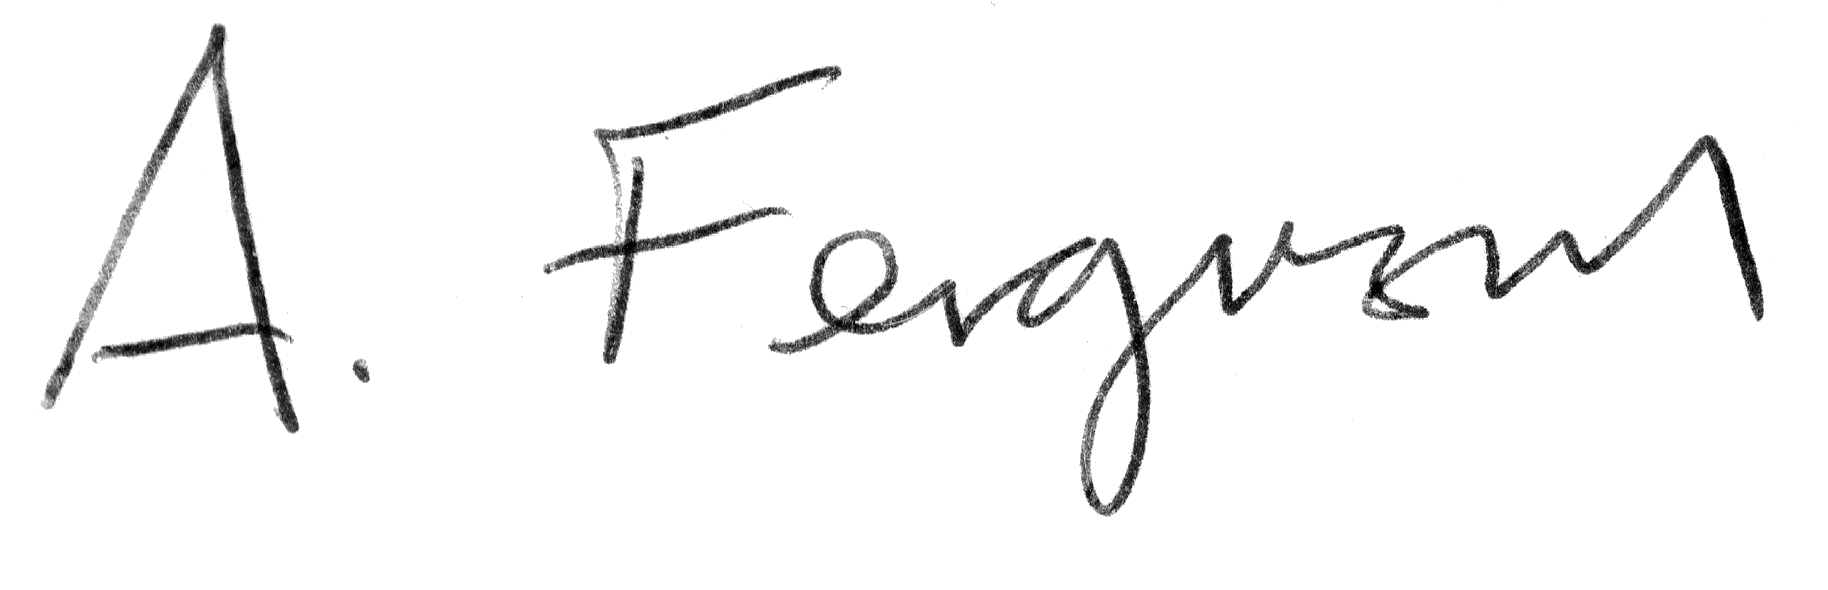
\includegraphics[width=0.2\textwidth]{signature_720}
%\vskip 0.65in % Whitespace between the signature text and your name
\\
\noindent
\fromsig
\vskip -0.05in
\titleone\\
\department\\
\institution\\
\vskip -0.1in
\noindent cc: M.S.~Jones, B.~Ashwood, A.~Tokmakoff
}

%----------------------------------------------------------------------------------------

\begin{document}

%----------------------------------------------------------------------------------------
%	TO ADDRESS
%----------------------------------------------------------------------------------------

\begin{letter}
{
Prof.\ Hanadi Sleiman \\
Associate Editor, \textit{The Journal of the American Chemical Society}
}

%----------------------------------------------------------------------------------------
%	LETTER CONTENT
%----------------------------------------------------------------------------------------

\opening{Dear Prof.\ Sleiman}

Thank you for your 6-Jul-2021 message regarding our article ``Determining sequence-dependent DNA oligonucleotide hybridization and dehybridization mechanisms using coarse-grained molecular simulation, Markov state models, and infrared spectroscopy'' assigned manuscript ID ja-2021-05219p. We thank you for handling our submission and the anonymous reviewers for their careful reading and critical assessment of our work.

We reproduce below the full text of the reviewer comments in blue along with our responses, reproduction of the changes made to our manuscript, and the locations of these edits. The modifications within our revised submission in response to the reviewer comments are indicated in red text. 

In light of these changes, we hope that our revised submission is suitable for publication in \textit{The Journal of the American Chemical Society}.

\closing{Yours Sincerely}

\end{letter}

%----------------------------------------------------------------------------------------

\clearpage
\newpage

\begin{shaded}
\textbf{Response to Reviewer \# 1}
\end{shaded}

\textcolor{blue}{In the manuscript ``Determining sequence-dependent DNA oligonucleotide hybridization and dehybridization mechanisms using coarse-grained molecular simulation, Markov state models, and infrared spectroscopy'', Jones et al. provide a well-designed and compelling study of DNA hybridization kinetics and dynamics that succinctly encompasses both experiment and theory. They demonstrate that the coarse-grained model of DNA, 3SPN.2, can not only well-reproduce the relative kinetic rates of sequence-dependent hybridization but also can reveal critical insights into their physical underpinnings. These insights are driven by the use of state-of-the-art applications of machine learning to Markov state model construction and well-validated with temperature jump infrared spectroscopy. In particular, the demonstration of how the placement of two G:C base pairs within the sequence can dramatically affect the energy landscape is truly impactful for the design of DNA sequences with desired properties. We believe this work is well suited for JACS publication after the Authors address a few major and minor points.}

\textbf{Author Reply:}   We thank the reviewer for their close reading of the manuscript and are pleased that they find the work impactful and suitable for publication in JACS.

\textcolor{blue}{Major point.
1)      Many of the core conclusions about the hybridization and dehybridzation mechanisms are based on the designation of the relevant metastable states as H, 5S2, 3S2, 5S4, F4, and D. While the authors do an excellent job of demonstrating that 2-6 state models provide an accurate description of the dynamics, in the current form, the paper does not provide sufficient evidence to support their chosen representative microstates and associated nomenclature (the only evidence being the ``representative'' structures shown in Figures 2A, C). A given macrostate represents an ensemble of microstates and it should be demonstrated that a significant fraction of the microstates that have a high probability of belonging to a particular macrostate share the same or similar base-pairing pattern. This would better justify how the authors chose to describe these states as 5S2, 3S2, etc., and provide the reader with more confidence that the mechanisms follow from the simulations. At the least, the authors should describe how the representative microstates (depicted in Figure 2A, C) were obtained.
}

\textbf{Author Reply:} The designation and structural representation of the macrostates is crucial to the core conclusions of the manuscript and we concur that we can and should better expose for the reader how the representative microstates were selected, how representative they are of the microstate ensemble within the macrostate, and our analysis of the base-pairing patterns within each macrostate that motivated our naming scheme.


On p.~19, we have added the following text:

``...each of these macrostates. \rood{The representative microstates emblematic of each macrostate were selected randomly from those possessing high ($>$99\%) macrostate membership probabilities. Since the microstate ensemble exhibits a range of conformations, however, it is useful to characterize the degree of structural heterogeneity to determine the degree to which these microstates are emblematic of the distribution. In Fig.~S5 we present a projection of our macrostates into two physical order parameters -- the degree of 3$^\prime$ shift and degree of 5$^\prime$ shift -- to provide an interpretable embedding of the macrostates that exposes base pairing patterns and structural heterogeneity within the microstate ensemble. In all cases, we find these microstate distributions to be relatively narrowly focused within the low-free energy core of each macrostate such that a single archetypal microstate is indeed a good representative for the ensemble and an accurate representation of the base pairing pattern of the macrostate.} In Fig. 2b we present...''

We also added the new Fig.~S5 to the Supporting Information where we discuss at some length within the caption the important issues raised by the reviewer. The figure and its caption are reproduced below.

\clearpage
\newpage

\begin{figure}[ht!]
	\centering
    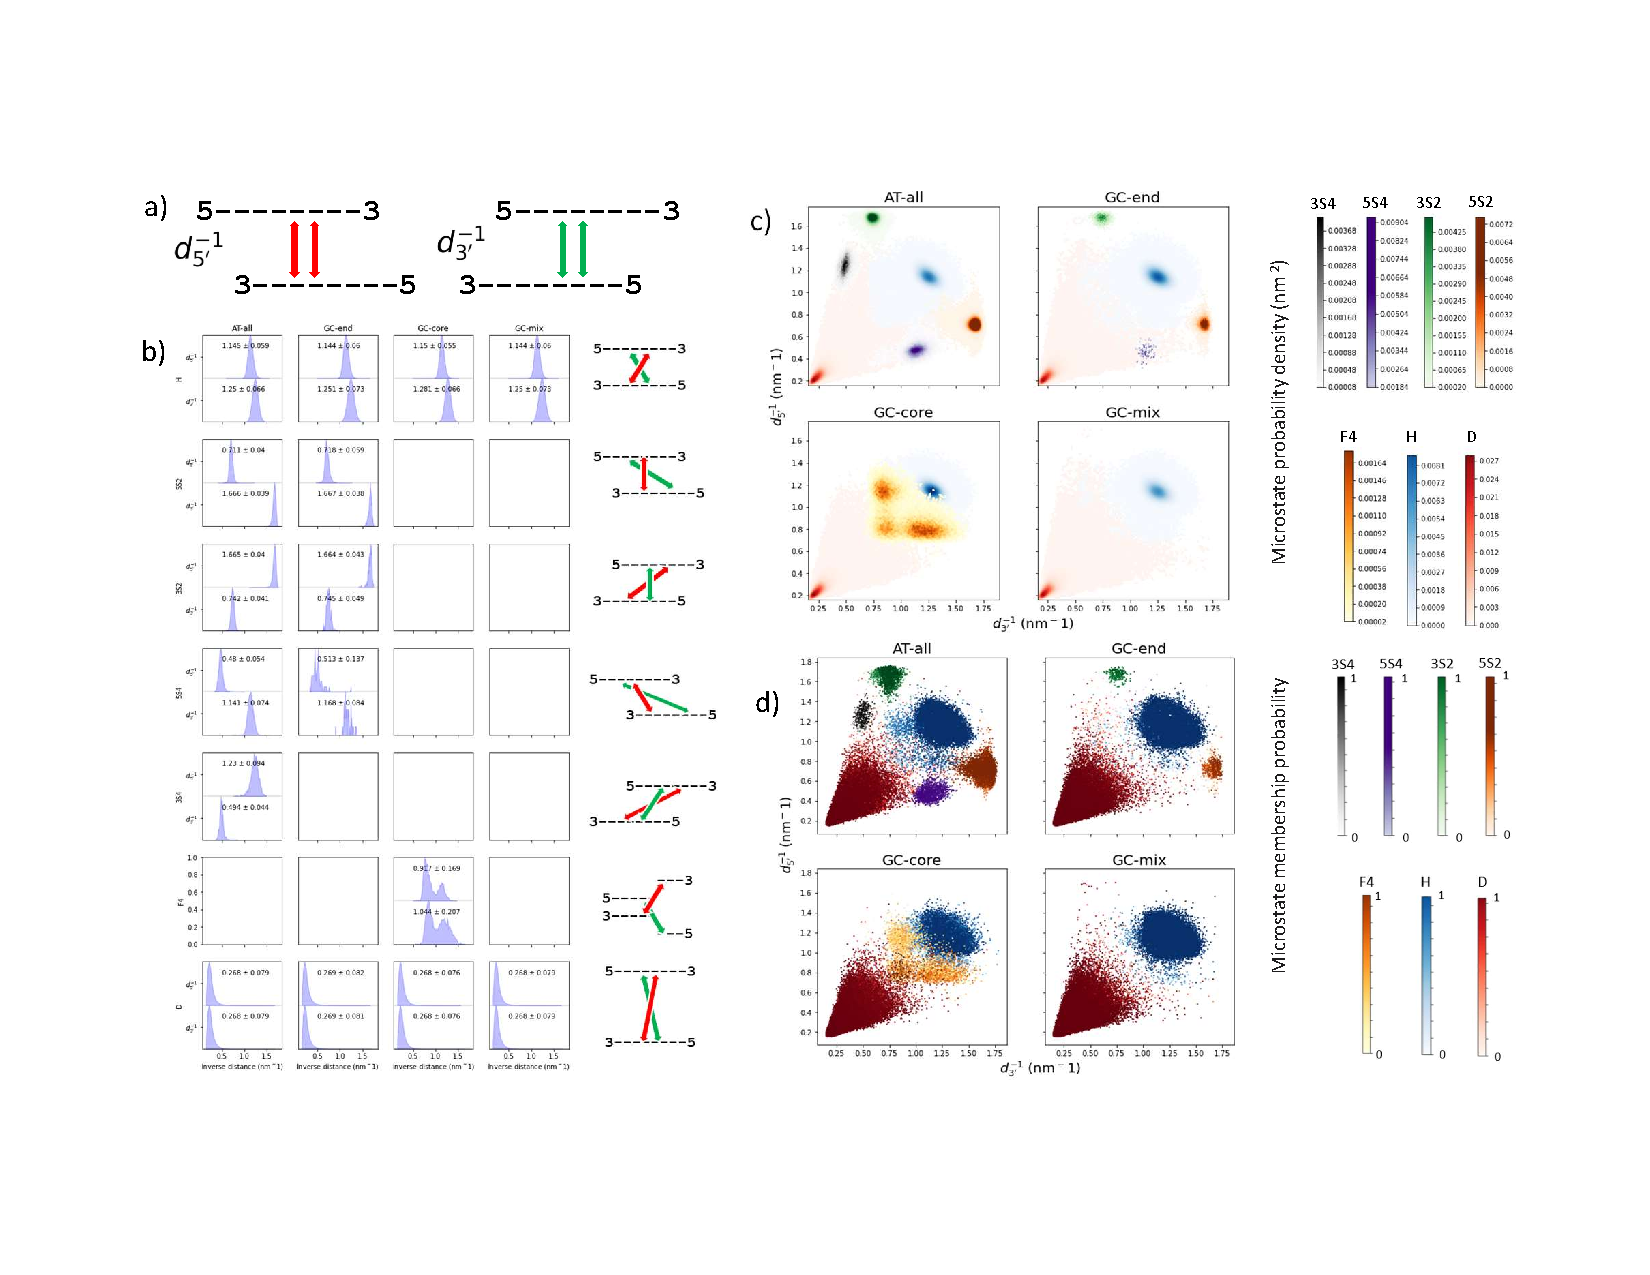
\includegraphics[angle=90,origin=c,width=1.0\textwidth]{../FigS5.pdf}
\end{figure}

\begin{figure}[ht!]
	\begin{center}
        \caption*{\textbf{Figure S5.}\rood{Macrostate interpretation and structural analysis. The Markov state model macrostates are learned from the simulation trajectories using the featurization and deep learning procedure described in Section 2.1.2 of the main text, but it is informative to perform a \textit{post hoc} projection of the simulation data into a low-dimensional space spanned by physically interpretable order parameters in order to determine the structural characteristics of each macrostate and the structural heterogeneity of the microstate ensemble. (a) Definition of two physically-interpretable order parameters useful in characterizing the structure and base pairing of each microstate under both shifting and fraying. We define the $3^\prime$ shift for a particular base on a strand as the linear distance between that base and the base on the complementary strand offset by two base pairs in the $3^\prime$ direction. This distance reaches a minimum when the two strands are mutually shifted two base pairs in the $3^\prime$ direction. We define $d_{3^\prime}$ as the mean $3^\prime$ shift averaged over the two central bases, represented by red arrows, in the complementary strands. It is more convenient to work the reciprocal $d_{3^\prime}^{-1}$, since it has a finite range whereas $d_{3^\prime}$ diverges for dehybridized strands. We define $d_{5^\prime}^{-1}$ analogously as the reciprocal mean $5^\prime$ shift, represented by green arrows. We have found this pair of variables extremely informative in revealing the microstate and macrostate structure and base pairing patterns. (b) We report the mean and standard deviation of $d_{3^\prime}$ and $d_{5^\prime}$ taken over all microstates comprising each macrostate for each sequence. The small standard deviations that are consistent with a narrow distribution of the bulk of the microstates around the free energy minimum of each macrostate. Cartoon renderings reflect the dominant configurations of each macrostate and how each is represented by the $d_{3^\prime}^{-1}$ and $d_{5^\prime}^{-1}$ order parameters green and red arrows, respectively. (c) Superposition of sample density for each macrostate for each sequence AT-all, GC-end, GC-core, and GC-mix projected into $d_{3^\prime}^{-1}$-$d_{5^\prime}^{-1}$. This panel conveys two important pieces of information. First, each macrostate is anchored around a single free energy minimum containing the preponderance of the probability mass of the microstate ensemble. These projections indicate a relatively narrowly peaked distribution of microstates around the free energy minimum with a broad tail. Second, the location of each macrostate free energy minimum in the $d_{3^\prime}^{-1}$-$d_{5^\prime}^{-1}$ projection readily illuminates the base pair pattern within the duplex. Within the fully hybridized H state (blue) $d_{3^\prime}^{-1}$ $\approx$ $d_{5^\prime}^{-1}$ $\approx$ 1.2 nm$^{-1}$. A 2 b.p.\ shift to 3$^\prime$ is manifest in a decrease in $d_{3^\prime}^{-1}$ (increase in $d_{3^\prime}$) and an increase in $d_{5^\prime}^{-1}$ (decrease in $d_{5^\prime}$) producing the stable 3S2 state (green). A further 2 b.p.\ shift to 3$^\prime$ results in a further decrease in $d_{3^\prime}^{-1}$ and also a decrease in $d_{5^\prime}^{-1}$ (back down to the same value as in the H state) to produce the 3S4 state (black). Analogous arguments apply to the 2 b.p.\ 5$^\prime$ shifted state 5S2 (orange) and 4 b.p.\ 5$^\prime$ shifted state 5S4 (purple). The dehybridized state D exists, due to the finite box size, at $d_{3^\prime}^{-1}$ $\approx$ $d_{5^\prime}^{-1}$ $\approx$ 0.2 nm$^{-1}$ (red). The GC-core frayed state F4 (orange) exists as a heart-shaped region between the H and D sates, with each symmetric lobe of the heart corresponding to fraying of one or other of the loose ends. (d) Coloring the microstates by their membership probabilities to their assigned macrostate under a fuzzy clustering procedure shows that microstates lying in the vicinity of the free energy minima have high probabilities whereas those at the macrostate cluster boundaries have less definitive assignments. The former comprise the preponderance of the microstate ensemble while the latter represent intermediate configurations that are transiently occupied as the system transitions from one macrostate to another.}}
        %\label{fig:macrostate_colors_FES}
	\end{center}
\end{figure}

\clearpage
\newpage



\textcolor{blue}{1)      It is unclear how five datasets were selected used for cross-validation in the SRVs (P. 10 L. 43). One would naively think a 50:50 split of a single trajectory would result in only one dataset. A bit more detail could be provided here.}

\textbf{Author Reply:}   Five-fold cross-validation was conducted by constructing five random partitions of the 40 independent trajectories into a training set of 20 trajectories and a validation set of 20 trajectories. This manner of splitting the data at the level of complete trajectories -- as opposed to splitting a single trajectory into multiple subtrajectories -- is desirable as it allows our SRV/MSM approach to learn over long 25 $\mu$s trajectories and infer slowly relaxing collective modes that may not be accessible within short sub-trajectories~\citep{Sidky2019High-ResolutionVAMPnets}. We have better clarified this procedure for the reader by revising the text on p.~11 to read: 

We guarded against overfitting using five-fold cross-validation in which we \rood{constructed five random partitions of the 40 independent simulation trajectories into a training set of 20 trajectories and a validation set of 20 trajectories}.\citep{Sidky2019High-ResolutionVAMPnets}




\textcolor{blue}{2)      For the validation of embedding dimensions (P. 11 L. 3), it is hard to judge the presence of a kink at 5D in the AT-all sequence since only a maximum of 6D is shown in Fig.~S1. Could a few additional dimensions be provided?}

\textbf{Author Reply:}   We agree that it is more difficult to see the kink for the AT-all sequence than the other sequences. As suggested by the reviewer, we added two additional modes to the cross-validation procedure that does indeed better expose this kink at five slow modes. We have updated the corresponding panel Fig.~S1 and also reproduce it below.

% Fig. S1
\begin{figure}[ht!]
	\begin{center}
        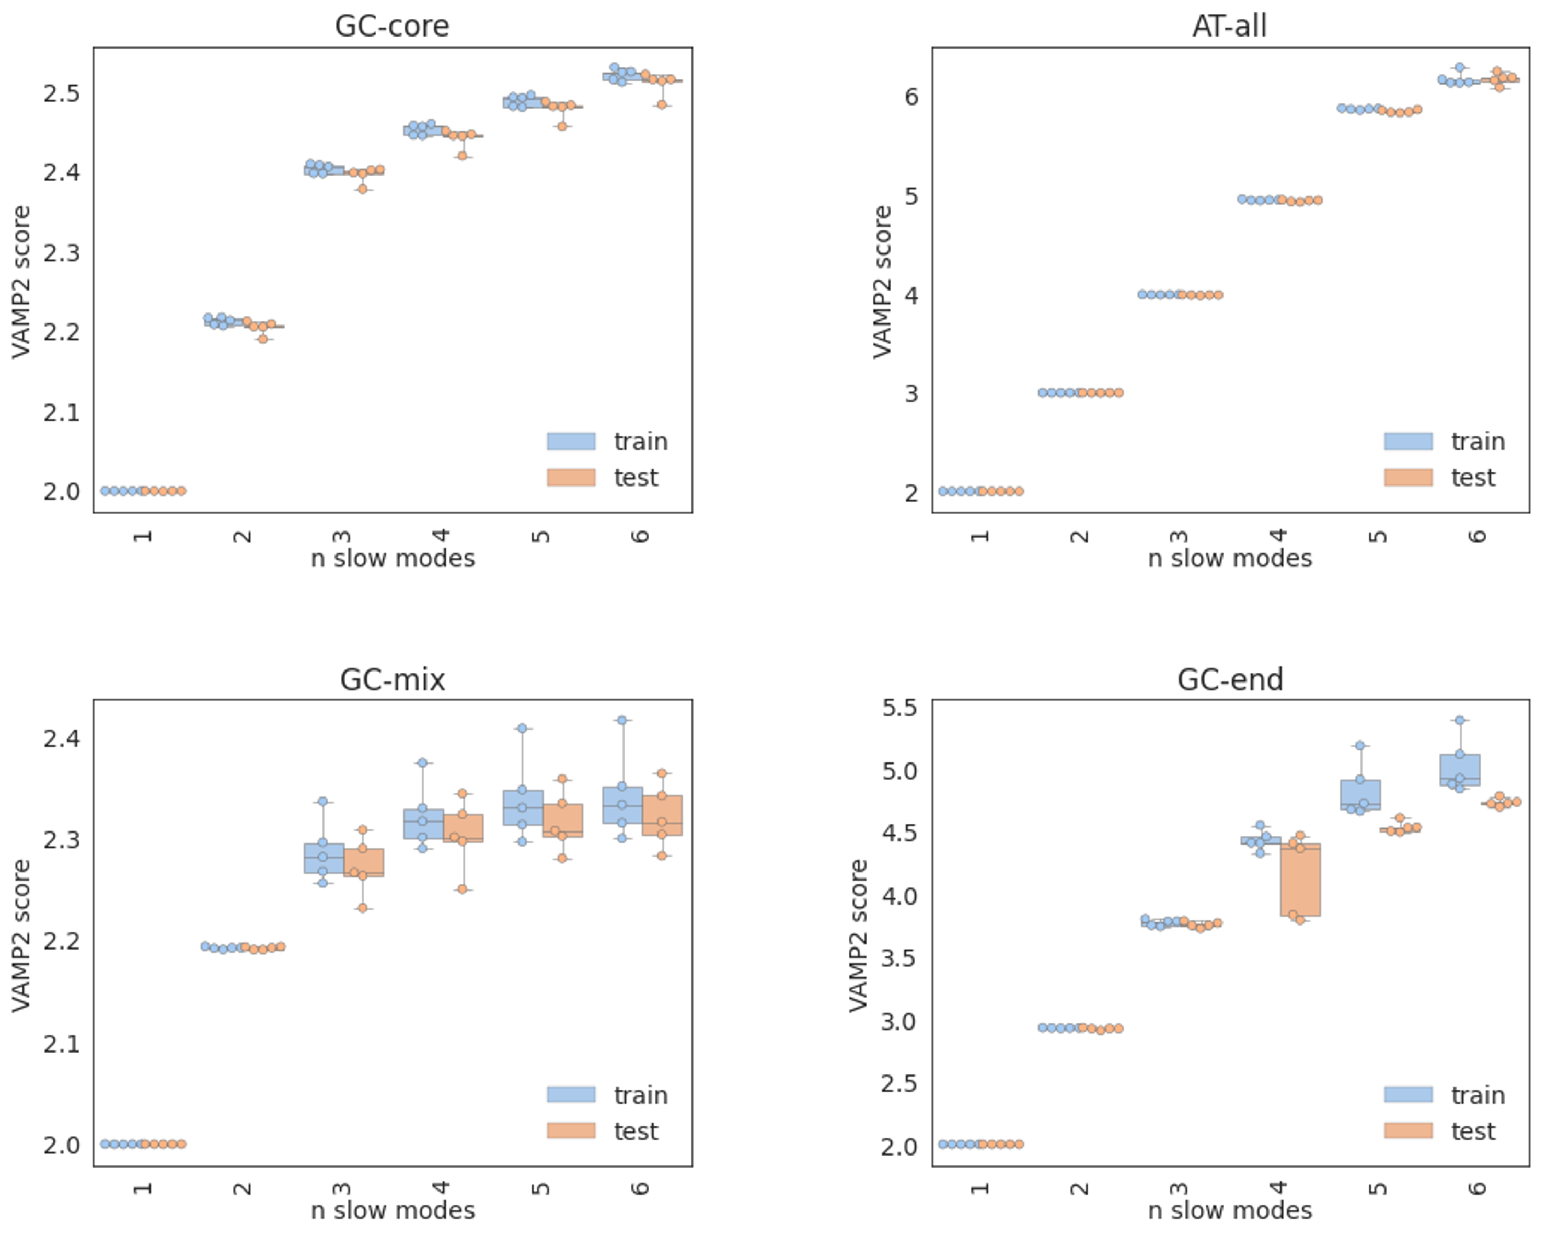
\includegraphics[width=0.8\textwidth]{../FigS1.pdf}
         \caption*{\textbf{Figure S1.}Five-fold cross-validation of the SRV VAMP-2 scores to select the optimal number of SRV coordinates for each sequence. A knee in the VAMP-2 plot was identified at the fifth, fourth, third, and second slow modes for AT-all, GC-end, GC-core, and GC-mix, respectively. An embedding of corresponding dimensionality was then used to cluster frames into discrete states. The absence of any significant separation in the training and testing VAMP-2 scores demonstrates that model is not overfitted.}
        \label{fig:SIFig1}
	\end{center}
\end{figure}



\textcolor{blue}{3)      The values associated with the ``slow'' and ``fast'' rates appear to be inverse quantities, but this is not mentioned in the text (P. 14 L. 44).}

\textbf{Author Reply:}   The reviewer is correct that the rates have units s$^{-1}$ and describe the inverse of the experimental timescales shown on page 15. We agree that the sentence on is unclear in its current form and have made the following change to that text on p.~15:

``We conducted T-jump IR experiments for each DNA sequence as a function of temperature and extracted \rood{the ``slow'' $k_d^\mathrm{slow}$  and ``fast'' $k_d^\mathrm{fast}$ rates, corresponding to processes proceeding on 10-30 $\mu$s and 70-100 ns timescales, respectively.''}




\textcolor{blue}{4)      In Figure 1 the units for rates are not provided.}

\textbf{Author Reply:}   Thank you for catching this error. Fig.~1 has been updated to include units in s$^{-1}$. 



\textcolor{blue}{5)      In the comparison between experiments and theory for slow and fast T-jump IR responses (P. 17 L. 9), were there any correlations between the goodness-of-fit in the calculated rates (Figure S4) and the agreement with experiments for a given system? It is hard to judge as is because the goodness-of-fit values were not provided with Figure S4.}

\textbf{Author Reply:}     We have updated all panels of Fig.~S4 plots to include $R^2$ values determined by linear least squares fits of the models in log-space (i.e., $\log \left( f \right) = -k_d t$) and have also re-plotted the data on log-linear axes for easier comparisons between the data and fits. The revised figure is reproduced below. In all cases except the lowest temperature T$_m$-5 K slow response fits where dissociation data is sparse, we report good fits with $R^2$ $>$ 0.88. We see marginally less good fits for the GC-core sequence compared to the other three systems, possibly -- as we observe in Section 3.1 of the main text -- due to its high propensity to fray, but the reduction in the quality of the fit is only marginal and in absolute terms the fits are still very good.


\clearpage
\newpage

% Fig. S4
\begin{figure}[ht!]
	\centering
    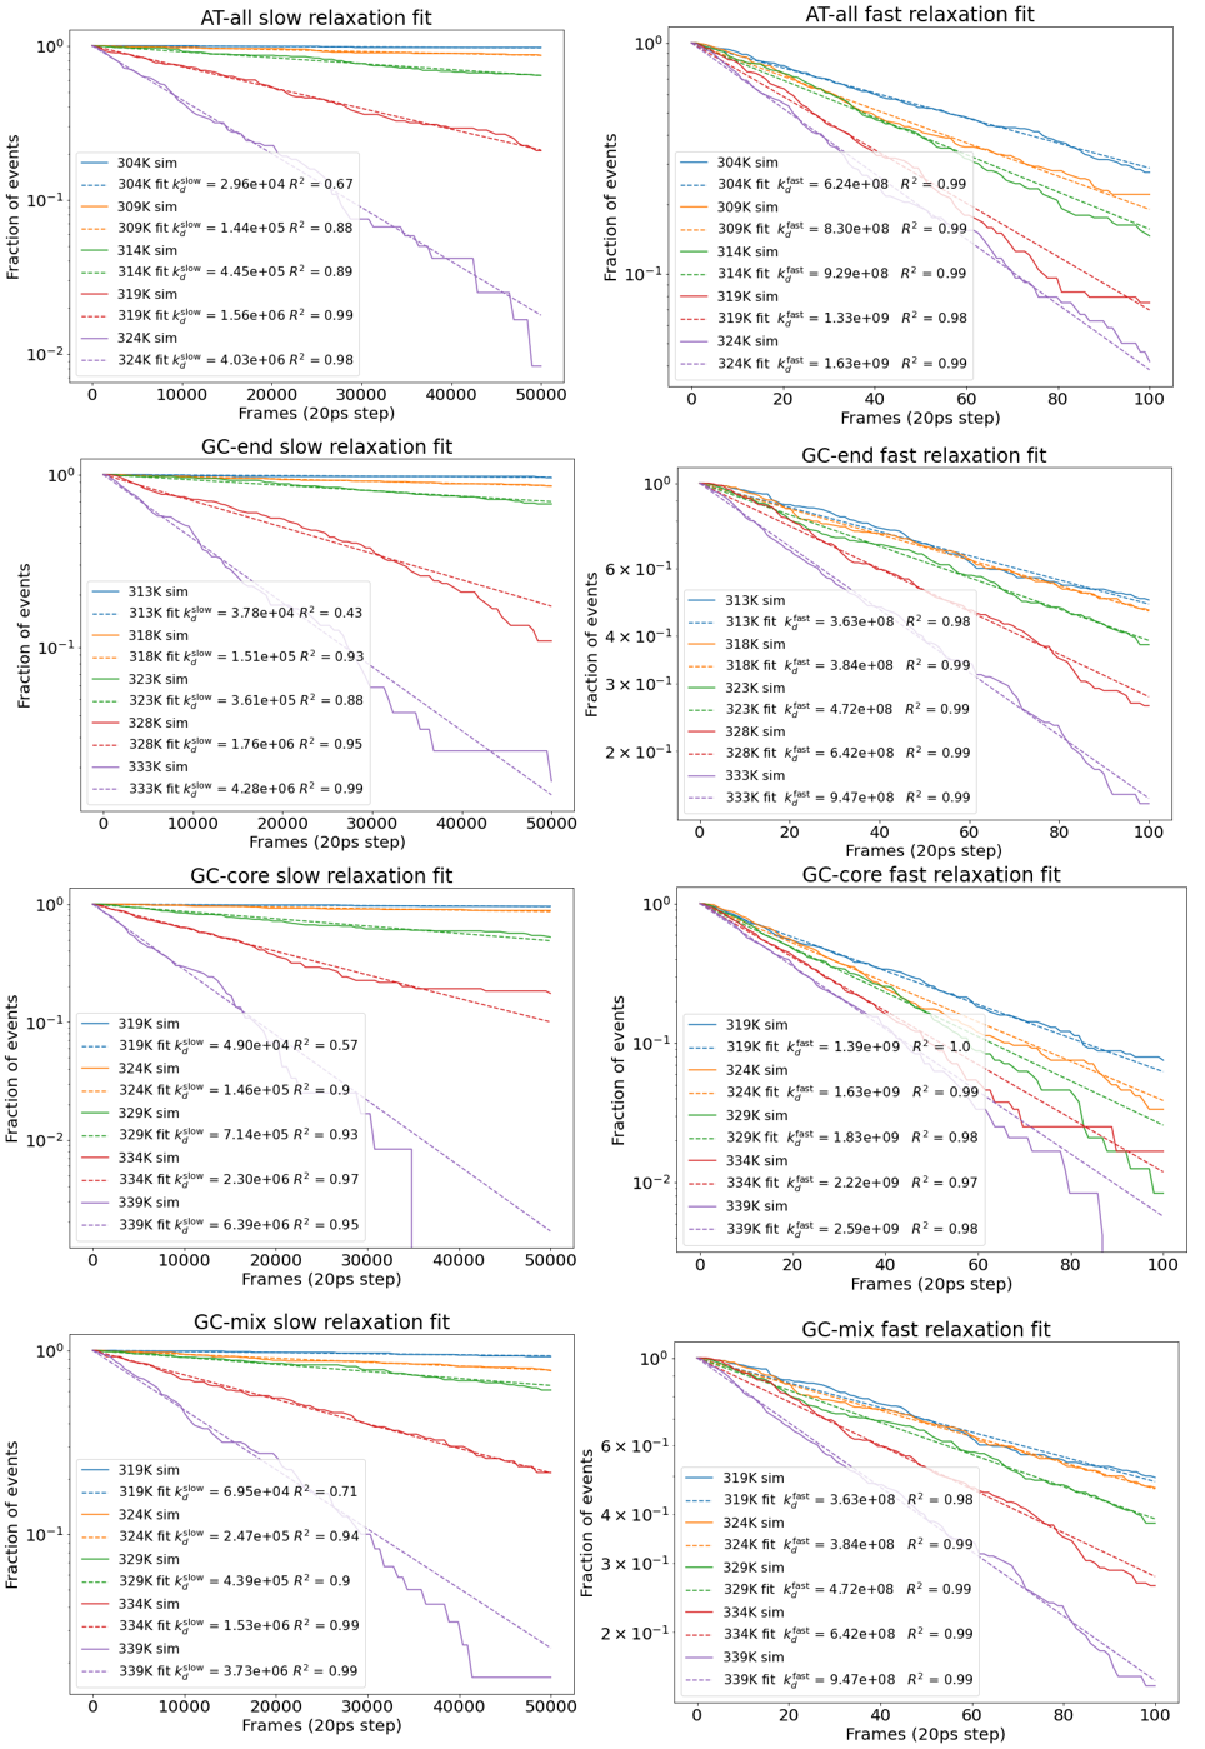
\includegraphics[width=.75\textwidth]{../FigS4.pdf}
   \caption*{\textbf{Figure S4.} Exponential fits for both slow (dissociation) and fast (fraying) response for all four sequences during ``computational T-jump'' experiments. From 120 independent 1 $\mu$s simulations, we compiled the slow response data by recording the fraction of sequences with both central Watson-Crick base pairs intact as a function of time, and the fast response data as the fraction of sequences with both terminal Watson-Crick base pairs intact as a function of time. We define a Watson-Crick base pair to be intact if the centers-of-mass of the two comlementary bases lie within a linear distance of 1.3 nm. We extracted our computational estimate of $k_d^\mathrm{fast}$ by fitting a decaying exponential to the fraction of bound A:T termini as a function of time $f_\mathrm{unfrayed}(t) = \exp(-k_d^\mathrm{fast}t)$. Similarly, we extracted our computational estimate of $k_d^\mathrm{slow}$ by fitting a decaying exponential to the fraction of hybridized sequences as a function of time $f_\mathrm{hybridized}(t) = \exp(-k_d^\mathrm{slow}t)$. \rood{We report within the figure legend of each panel the coefficient of determination $R^2$ for a least squares linear fit of the model to the data in log space (i.e., $\log \left( f \right) = -k_d t$) and data are plotted on log-linear axes to facilitate visual comparison of the fits. In all cases we observe excellent fits of the models to the data with all $R^2$ > 0.88 except for the slow response at the the lowest temperature T$_m$-5K where dissociation events are sparse.}}
    \label{fig:SIFig4}
\end{figure}

\clearpage
\newpage




\textcolor{blue}{6)       The authors chose to compute the temperature jump relaxation rates from fits to quantities obtained directly from the MD simulation. However, it is not clear why the authors did not also compute the relaxation of observables from estimated Markov state models following (P. N. A. S. USA. 2011;108(12):4822-4827). This approach has also been previously used to compare kinetics obtained from Markov state models with other spectroscopic temperature-jump based experiments in DNA (J. Phys. Chem. B. 2019;123(10):2291-2304.) and RNA (J. Chem. Theory Comput. 2017;108(2):926-934) oligomers which should be mentioned. If possible, it would be interesting to compare or discuss the differences between their approach and these previous approaches.}


\textbf{Author Reply:}   The reviewer raises an important point regarding the dynamical fingerprinting methodology that have been developed to compare MSM predictions and relaxation experiments. We are familiar with these techniques and, in fact, are currently applying them in our current work on abasic DNA. We did attempt to apply them in the present work, but these analyses proved less informative than we had hoped due to two primary factors. 

First, the experimental data contains fast responses occurring on time scales of $\sim$100 ns. As detailed in Section 3.1 and Figure 1, these fast motions occur in our simulations at an acceleration factor of approximately 120$\times$ and so proceed on a time scale of $\sim$1 ns. As such, these motions lie below the $\tau$ = 1.2 ns lag time used to construct our MSMs that is required to converge the leading slow modes and produce a Markovian model capable of passing the Chapman-Kolmogorov test (cf. Figs.~S2-3). As such, we cannot draw comparisons of our MSM against the fast experimental data. 

Second, the dynamical fingerprinting method provides an elegant means to compare experimental data against an MSM constructed at the same state point (e.g., temperature, pressure, salt concentration). We constructed only a single MSM for each sequence at the melting temperature of the 3SPN.2 model that required the collection of 1 ms of simulation data for each sequence in order to observe sufficiently many hybridization/dehybridization events for robust fitting of the model parameters (Section 2.1.1). The experimental relaxation data, however, was collected over a range of temperatures and we wished to make comparisons across this entire experimental range. Fitting additional MSMs was too computationally burdensome due to the high volume of data required and the cost of these simulations, so instead we conducted 120 $\times$ 1 $\mu$s simulations for each DNA sequence at each temperature. These trajectory data were too sparse to fit a robust MSM, but did allow us to make a direct comparison between the MD simulations and the experimental measurements over the full temperature range. 

We therefore elected to structure our manuscript such that we first test the MD simulation predictions against experimental data in Section 3.1, then, after having validated the simulation data upon which the MSMs are constructed, perform MSM construction and analysis in Sections 3.2-6. Finally, in Section 3.7 we close with a test of a specific prediction of our MSM (the existence of long-lived metastable shifted states) that was amenable to comparison against T-jump IR.

We concur with the reviewer that we can and should explicitly mention dynamical fingerprinting approach and provide some discussion for the reader why we did not employ this approach in the present study. To this end, we have added the following text to the end of Section 3.1 on p.~18:

``fast kinetics of the four DNA oligomers\rood{, and lends confidence in the use of these data for the parameterization of Markov state models of the long-time dynamics of each sequence. We observe that the dynamical fingerprinting approach presents an elegant means to compare experimental relaxation data directly against a Markov state model extracted from simulation data in terms of a ``fingerprint'' of peaks with amplitudes and time scales related to the relaxation of particular system observables~\citep{Noe2011DynamicalExperiments}. These techniques have been previously employed to in applications to base stacking of DNA dinucleoside monophosphates~\citep{Remington2019MolecularKinetics} and RNA~\citep{Pinamonti2017}. We explored the use of this approach to validate the MD simulation data but encountered challenges in resolving fast dynamical motions below the lag time of the fitted MSM and the extremely high computational cost of collecting sufficient simulation data to fit MSMs at each temperature for which experimental data was collected. Accordingly, we instead elected to perform a direct comparison between the experimental data and MD trajectories to validate the simulations themselves, then proceed to train MSMs over these data and conduct analysis and experimental tests of the MSM predictions.}''






\clearpage
\newpage

\begin{shaded}
\textbf{Response to Reviewer \# 2}
\end{shaded}

\textcolor{blue}{This paper reports simulation results on the hybridization and dehybridization mechanisms near to the melting temperature of a number of short DNA sequences, and accompanying temperature jump IR experiments. The sequences are chosen to have a repeating AT motif that potentially allows relatively stable out-of register duplex states, with a focus being on how these states are disrupted, by the presence of GC base pairs. The authors show that the introduction of just 2 appropriately-positioned base pairs can change the kinetics to a simple two-state behaviour from one in which multiple states contribute.}

\textcolor{blue}{I found this an interesting study that nicely illustrated some of the potential effects of sequence on (de)hybridization mechanisms. However, I found the results unsurprising, and these types of effects have been previously explored in the literature. Although I can't therefore recommend publication in JACS, I think it would be very appropriate for one of the more specialized ACS journals.}

\textbf{Author Reply:}  We are pleased that the reviewer finds our results interesting and suitable for publication. We concur with the reviewer that this work builds upon prior studies in the literature on sequence effects upon hybridization/dehybridization mechanisms, but we contend that it goes beyond these studies in presenting a means to rigorously resolve and quantify these dynamics. The primary novelty and impact of this work lies less in the discovery of the particular metastable states, but in furnishing quantitative and predictive kinetic models of the dynamical transition network between these states that furnishes experimentally testable predictions and new understanding and quantification of the influence of sequence upon thermodynamics and kinetics.

We better contextualize the scope and impact of our work in the final sentence of the Abstract:

``Our results establish new understanding of the dynamical richness of sequence-dependent kinetics and mechanisms of DNA hybridization/dehybridization \rood{by furnishing quantitative and predictive kinetic models of the dynamical transition network between metastable states}, present a molecular basis with which to understand experimental temperature jump data, and furnish foundational design rules by which to rationally engineer the kinetics and pathways of DNA association and dissociation for DNA nanotechnology applications.''

and we go on to state in the Introduction:

``Out-of-register ``shifted'' base paired structures \citep{Flamm2000RNAResolution, Romano2013DNADependence, Hinckley2014Coarse-grainedEffects, Maciejczyk2014DNAModel, Araque2016LatticeCooperativity, Xiao2019} and frayed structures \citep{Zgarbova2014BaseRNA, Nonin1995TerminalFraying, Nikolova2012ProbingSimulations, Andreatta2006UltrafastHelix} stand as candidates for metastable states with the potential to mediate substantial deviations from all-or-nothing behavior, but the degree to which these states are kinetically relevant is difficult to determine experimentally and is likely to be highly sequence-dependent.''

``We validate the new computational models of hybridization/dehybridization dynamics developed in this work against new experimental data and reinterpret our prior experimental observations in light of the new computational understanding. Consistent with previous studies, \citep{Hinckley2014Coarse-grainedEffects,Romano2013DNADependence,Araque2016LatticeCooperativity} we find the degree of repetitiveness in the sequence -- and therefore the kinetic accessibility and thermodynamic stability of out-of-register shifted states -- leads to richer dynamics populated by a diversity of long-lived metastable states. Our data-driven modeling and analysis rigorously quantifies these behaviors and furnishes accurate predictive models of the hybridization/dehybridization rates, dynamical pathways, and metastable states. Specifically, we demonstrate that disrupting repetitive stretches of A:T bases by placement of interrupting G:C base pairs enables us to tune the landscape from rich six-state to simple two-state ``all-or-nothing'' behavior, and the specific location of the interrupting pair can be used to modulate the stability of long-lived frayed states.''

``Taken together, our analyses establish new molecular-level understanding of the sequence-dependent kinetics and pathways through quantitative predictive models for the long-time system dynamics, resolution of the dynamical folding pathways and metastable states, and elementary design rules with which to control the dynamical behaviors of the system. We anticipate that this new foundational understanding, and the extension of our approach to more extensive families of DNA sequences, can guide the rational design of DNA oligomers with tailored kinetic properties engineered for DNA nanotechnology applications such as DNA-PAINT. \citep{Shah2019, Strauss2020UpDNA-PAINT}'' 




\textcolor{blue}{One limitation of the study is its reliance on ``brute-force'' simulations (rather than using advanced sampling/rare-event techniques) to probe the transition. This means that systems of very high concentration (7 M) and temperatures close to the melting point have to be used, which are probably not the conditions of most interest.}

\textbf{Author Reply:}    (I) We agree with the reviewer that it may be possible to use biasing techniques in order to efficiently collect the data required to construct the MSMs. We are very familiar with the use of such techniques and another major interest of our research group is iterative strategies to perform data-driven determination of collective variables from simulation trajectories, enhanced sampling in these variables, and then estimation of new and improved collective variables from the enhanced sampling trajectories \citep{Sidky2020MolecularSimulators, Sidky2020MachineSimulation, Chen2019CapabilitiesSystems, Chen2019NonlinearVAMPnets, Phys2018CollectiveDesign, Chen2018MolecularExploration}. In the present work, we chose not to employ biased simulations and instead collect unbiased trajectories for three main reasons. 

First, the 3SPN.2 coarse-grained DNA model is sufficiently inexpensive that it was possible to collect adequate unbiased simulation data to parameterize robust MSMs at reasonable costs. As we state on p.~8: 

``Each simulation was conducted for 26 $\mu$s and frames saved to disc every 100 ps. Each simulation required $\sim$24 CPU-hours on 28$\times$Intel E5-2680v4 CPU cores. The first 1 $\mu$s of each run was discarded for equilibration providing us with 40$\times$25 $\mu$s = 1 ms of simulation data for each sequence, during which time we observed 55-100 hybridization/dehybridization events.''

Second, the unbiased simulation data are in good agreement with trends in experimental T-jump IR measurements of fast and slow relaxation responses (Section 3.1) and are sufficient to furnish robust, low-variance, and well-converged MSMs (Section 3.2, Figs.~S1-3). This indicates that the data are of sufficient quality and volume to present favorable experimental comparisons and learn reliable long-time kinetic models.

Third, although it is straightforward to correct biased simulation data to recover the unbiased thermodynamics, it is more challenging to recover the unbiased kinetics. Although a number of approaches do exist, it has been our experience that the kinetic corrections can present difficulties in numerical convergence. That is not to say that we could not have successfully applied this methods, but just that we did not have cause to do so since the unbiased data were not unreasonably expensive to collect and showed favorable experimental comparisons and produced robust MSMs.

We did note the possibility of performing biased simulations in the Introduction on p.~4-5, and have now elaborated these remarks to better explain our choice to proceed with unbiased simulations:

``The effect of the applied bias upon the thermodynamics can be rigorously corrected for using standard reweighting techniques \citep{Gallicchio2005TemperaturePaths, Souaille2001ExtensionCalculations, Shirts2008StatisticallyStates, Kumar1992THEMethod}. \rood{Rigorous elimination of the bias in the kinetics is critical for the construction of robust and reliable Markov state models that reflect the true system dynamics and are uncontaminated by any residual effects of the biasing potentials used to induce good sampling. A number of approaches to correct the kinetics are also available, including Girsanov reweighting, transition-based reweighting analysis (TRAM), dynamic histogram analysis method (DHAM), and their derivatives~\citep{Prinz2011OptimalDynamics, Chodera2011DynamicalTemperatures, Stelzl2017DynamicSimulations, Donati2017GirsanovModels, Donati2018GirsanovSimulations, Quer2018ANCOORDINATES} \citep{Mey2014XTRAM:States}. The application of these methods under the conditions of high bias necessary for good sampling can, however, present challenges for numerical convergence.} A number of coarse-grained DNA force fields have been developed that enable direct observation of these events over microsecond time scales via unbiased coarse-grained molecular dynamics simulations, \citep{Romano2013DNADependence, Hinckley2013AnHybridization, Maciejczyk2014DNAModel, Markegard2015, Dans2016MultiscaleDNA} which, up to an acceleration factor associated with the smoothing of the underlying free energy landscape inherent to the coarse-graining procedure, can preserve a faithful model of the unbiased dynamics and associated pathways. These models have previously been used to study biological phenomena such as nucleosome dynamics\citep{Lequieu2016Tension-dependentUnwrapping, Lequieu2017InSliding} and transcription factor binding \cite{Terakawa2015P53Simulations, Tan2018DynamicData} as well as nanotechnology applications such as strand displacement \citep{Srinivas2013OnDisplacement, Haley2020DesignDisplacement} and DNA origami \citep{Snodin2019Coarse-grainedOrigami, Doye2020TheOrigami}. \rood{In this study, we choose to employ a coarse-grained model for DNA \citep{Hinckley2013AnHybridization} that is sufficiently inexpensive to enable the collection of sufficient volumes of unbiased simulation trajectories and adequately sample configurational space that we do not need to appeal to biasing strategies to enhance convergence nor apply any \textit{post hoc} corrections to the thermodynamics or kinetics.}''

(II) Our specification of a single strand concentration of 7 mol/L in Section 2.1.1 on p.~7 was an (embarrassing) typo -- the true concentration is actually 7 mmol/L (i.e., 7 mM). This is only 3.5$\times$ higher than the 2 mmol/L experimental concentration, and so is actually quite a good approximation for the experimental conditions. We regret our error, and have corrected this text to now read:

``A single pair of self-complementary sequences were placed in a cubic periodic box with side length 7.8 nm corresponding to a single-strand concentration of \rood{7 mM}. \rood{This concentration is only 3.5$\times$ larger than the 2 mM concentration employed in our experimental analyses (Section 2.2).}''

(III) Finally, we deliberately chose to explore the melting temperature as the state point at which the hybridized and dehybridized populations are in balance and sought to probe the mechanism and kinetics of the hybridization/dehybridization transitions under these equilibrium conditions corresponding to no net thermodynamic preference for either state (i.e., minimally driven conditions). A favorable side effect of this choice was indeed that we observe approximately equal numbers of hybridization and dehybridization events in a single (sufficiently long) simulation, whereas temperatures away from $T_\mathrm{melt}$ would favor one over the other. It is an interesting question to consider how the mechanism and kinetics of hybridization/dehybridization may change with temperature. Exploring small excursions either side of $T_\mathrm{melt}$ may still be possible using unbiased simulations, but we concur with the reviewer that biased sampling would be required to observe sufficient numbers of hybridization (dehybridization) events at large excursions above (below) $T_\mathrm{melt}$.

In response to this point, we have modified text in the terminal paragraph of the Conclusions on p.~38 observing that this may be an interesting point for follow-up study:

``Going forward, we will extend this work to discern more general trends in sequence-dependent hybridization/dehybridization for a wider range of oligomer sequences and motivate strategies for experimental comparisons. \rood{We also suggest that the MSM approach followed in this work, possibly coupled with biased sampling and reweighting techniques \citep{Wu2014StatisticallyStates, Scherer2015PyEMMAModels}, may be well-suited to expose changes in the hybridization/dehybridization mechanism and kinetics as a function of temperature.}''


\textcolor{blue}{Very small points:
+ p16 line 3: "Although the 3SPN.2 model reproduces melting temperatures relatively well, we observed a systematic 4 K under-prediction relative to experiment and so we apply a universal (+4) K corrective calibration to our computational results". This sentence confused me at first. I presume you are just shifting your simulated kd slow curves to better match experiment, rather than shifting the data so that the melting temperatures agree. You may want to be more explicit as I read it as the latter at first. (Note one shouldn't expect the melting temperatures to agree as very different concentrations are being used in simulation and experiment, and one also has to correct for finite-size effects when estimating melting points from single duplex simulations (https://doi.org/10.1088/0953-8984/22/10/104102)}

\textbf{Author Reply:}   (I) We regret our lack of clarity in our choice of wording. Yes, we simply shifted the $k_d$ curves by a universal temperature shift, determined empirically to be +4 K, that produced the optimal match with the experimental data. 

We have also reworded the unclear wording regarding the temperature correction in Section 3.1 p.~17 to now read:

``Although the 3SPN.2 model reproduces melting temperatures relatively well, we observed a systematic 4 K under-prediction relative to experiment and so we apply a \rood{universal (+4) K corrective temperature shift} to our computational results.''

(II) We regret our erroneous reporting of a 7 M rather than 7 mM concentration as detailed in our previous response. As we have now clarified, our simulations and experiments are conducted at similar concentrations (7mM and 2 mM, respectively). We agree that we still cannot expect perfect agreement in the melting temperatures due to the residual small  difference in concentrations, but likely this is small in comparison to discrepancies introduced by the approximations inherent in the coarse-grained molecular model.

(III) We greatly appreciate this comment and suggestion to apply a fluctuation correction to our data in order to correct for artifacts associated with finite-size effects following the approach detailed in Ref.~\citep{Ouldridge2010ExtractingSimulations}. We have reanalyzed our slow repsonse data under the homodimer correction and this has pleasingly resulted in a slightly improved agreement between our simulations and experiment. The revised figure is reproduced below. 


\begin{figure}[ht!]
	\begin{center}
        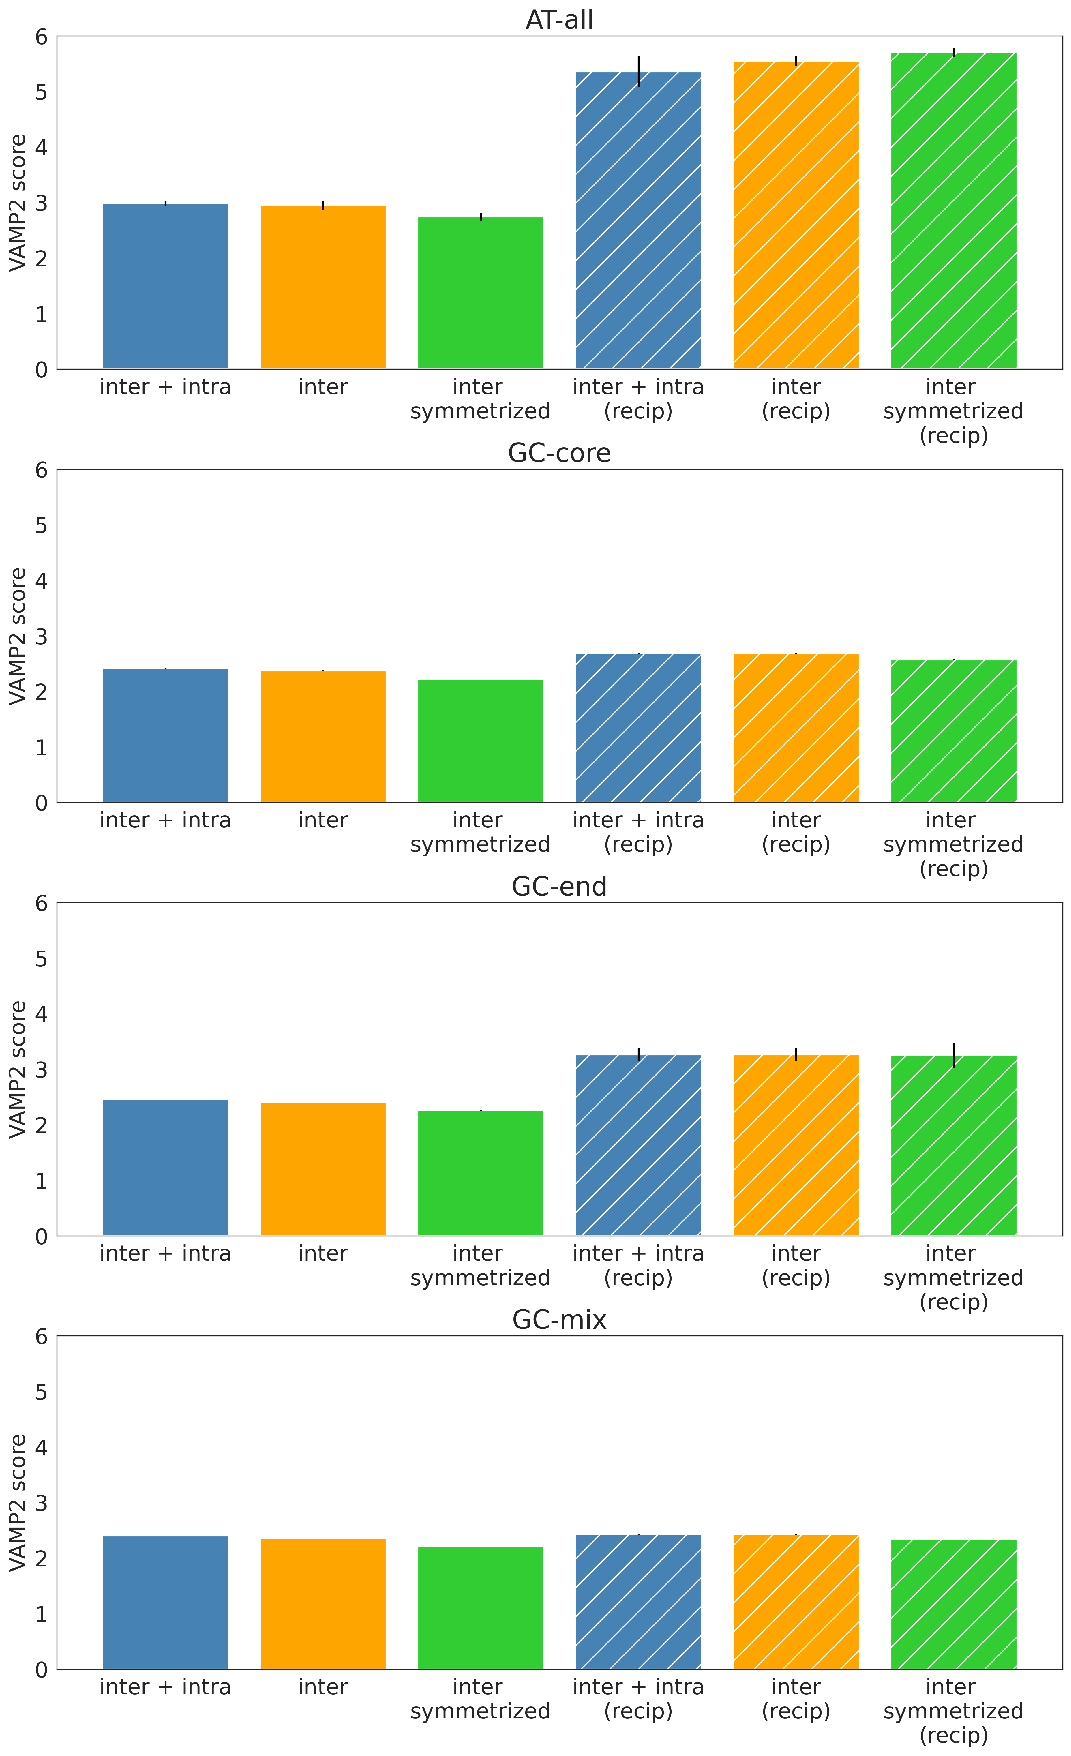
\includegraphics[width=0.8\textwidth]{../Fig1.pdf}
        \caption*{\textbf{Figure 1.} Experimental measurements and computational predictions of slow and fast at T-jump IR responses. Results are reported in terms of the final T-jump temperature. (a) The experimental and simulated slow rate constants $k_d^\mathrm{slow}$ corresponding to duplex dissociation over long time scales. \rood{We apply a fluctuation correction proposed by Ouldridge et al.\citep{Ouldridge2010ExtractingSimulations} to account for finite-size effects and ensure an asymptotically correct dimer fraction at long times.} (b) The experimental and simulated fast rate constant $k_d^\mathrm{fast}$ corresponding to terminal base-pair fraying on short time scales. The simulation results are corrected by a sequence-independent scaling factor that corrects for a 10$\times$ acceleration of the slow dissociation dynamics and 120$\times$ acceleration of the fast fraying dynamics. The simulated temperature in all cases is subjected to a (+4) K corrective calibration to account for an observed systematic under-prediction of the melting temperature by the 3SPN.2 model}
        \label{fig:relaxation-comparison}
	\end{center}
\end{figure}


In light of this modification, we have also added the following text to the Section 3.1 on p.~16: 

\rood{To correct for finite-size effects associated with the simulation of a single duplex within a periodic simulation box and ensure that we will observe asymptotically correct behavior at long times, we apply the fluctuation correction proposed by Ouldridge et al.\citep{Ouldridge2010ExtractingSimulations} to our predictions for $f_\mathrm{hybridized}$ bulk yields. We correct the values observed in our simulations $f_\mathrm{hybridized}^\mathrm{sim}$ to the bulk corrected result $f_\mathrm{hybridized}$ as,}

    \begin{equation}\label{}
    \phi = \frac{f_\mathrm{hybridized}^\mathrm{sim}}{1 - f_\mathrm{hybridized}^\mathrm{sim}}
    \end{equation}
    
    \begin{equation}\label{}
	f_\mathrm{hybridized} = (1+\frac{1}{4\phi}) - \sqrt{(1+\frac{1}{4\phi})^2 - 1}
	\end{equation}
	

Finally, we have also edited the following text in Section 3.1 on p.~17 to clarify that the fluctuation correction is only applied for the purposes of the experimental comparison in Section 3.1 and is not propagated throughout the remainder of the paper:

``The computational time scales and melting temperatures reported in the remainder of the paper are not corrected \rood{by these calibration corrections or finite-size fluctuation corrections} since we are only interested in the relative trends in the behaviors of the four sequences.''


\textcolor{blue}{+ p15 line 20 "beyond with" -> "beyond which"}

\textbf{Author Reply:}    This typo has been corrected.








\clearpage
\newpage

\begin{shaded}
\textbf{Response to Reviewer \# 3}
\end{shaded}

\textcolor{blue}{Jones et al present a combined experimental and computational paper that probes the dynamics of the DNA hybridization/de-hybridization transition. Through a Markov state model analysis of coarse-grained simulation, the authors identify states that contribute to the process, and present experimental evidence to support the role of these states. In particular, repetitive sequences are observed in simulations to have a number of misaligned states that are both appreciably stable and contribute to hybridization and de-hybridization pathways as intermediates. The role of these states is diminished by base pairs that disrupt the repetitive sequence. In the special case of a sequence with a strong core and weaker extremities, metastable "frayed" states are also observed. The presence of these states is assessed experimentally trough the analysis of relaxation timescales observed in T-jump IR spectroscopy; fast relaxation is attributed to fraying equilibria, and a broader fast relaxation to an increased heterogeniety due to the presence of mis-aligned intermediates.}

\textcolor{blue}{The paper is generally well-written, and, I believe, represents a good attempt to tackle this important process. I personally have had a manuscript "desk-rejected" by JACS on the basis that it is "too focussed on DNA biotechnology", and "primarily of interest to RNA and DNA chemists". The same statements could be made about this paper. However, I disagree with the conclusion that such papers are not appropriate for JACS. I would therefore recommend publication, subject to satisfactory responses to the comments below.  }

\textbf{Author Reply:}   We are delighted by the reviewer's warm reception of our paper, and pleased that they find it to be appropriate for publication in JACS.



\textcolor{blue}{1.   I was frequently confused as to the temperatures used in the experiments and analysis. At one point, it is noted that simulations are performed at melting temperatures. However, simulations are actually performed at a range of temperatures and it isn't always clear when looking at a figure which temperatures were used for simulation, NN model comparison or experiments (see eg. Figs 2 and 3 and 5). I would recommend noting the temperature used to obtain the data in each case.}

\textbf{Author Reply:}   We thank the reviewer for this suggestion and regret our lack of clarity in this matter. All simulations performed in this work were conducted at the melting temperature, with the exception of the simulations discussed in Section 3.1 where we consider a range of temperatures in order to draw comparisons to experimental measurements over this temperature range. We have added a number of clarifications to the text in order to more clearly convey this important point to the reader.

In Section 2.1.1 of the Methods on p.~7, we have added:

``\rood{With the exception of the simulation data reported in Section 3.1 where we draw comparisons against experimental data collected over a range of temperatures,} each sequence was simulated at its melting temperature -- AT-all: 309 K, GC-end: 317 K, GC- core: 324 K, GC-mix: 324 K -- in order to maximize the number of spontaneous transitions between dissociated and hybridized states.''

In Section 2.1.2 of the Methods on p.~9, we have added:

``In this work, MSMs were constructed for each of the four DNA sequences \rood{at their respective melting temperatures} from the 40$\times$25 simulation trajectories following a four-step protocol...''

In the first sentence of Section 3.3 on p.~21, we have added:

``We first compare the thermodynamic predictions for the equilibrium macrostate probabilities \rood{made by the MSM models fitted at the sequence melting temperatures} to those of the nearest neighbor (NN) model as a popular empirical model of DNA hybridization thermodynamics.''

In the first sentence of the caption of Fig.~2, we have added:

``Thermodynamic and kinetic predictions of the sequence-specific MSMs \rood{fitted at the sequence melting temperatures} for AT-all, GC-end, GC-core, and GC-mix.''

In the first sentence of the caption of Fig.~3, we have added:

``Comparison of the macrostate free energy predictions of the MSMs and nearest neighbor (NN) thermodynamic model \rood{at the sequence melting temperatures}.''

In the first sentence of Section 3.4 on p.~26, we have added:

``In addition to thermodynamic stabilities, the macrostate MSM also furnishes quantitative and interpretable predictions of hybridization and dehybridization pathways and mechanisms \rood{at the sequence melting temperatures}.''

In the second sentence of the Conclusions in Section 4 on p.~36, we have added:

``We conducted 1 ms of unbiased coarse-grained molecular dynamics simulations \rood{at the melting temperature of each sequence} and...''






\textcolor{blue}{2. P7 line 13 - surely these simulations were not really done at 7M? That sounds impossibly dense.}

\textbf{Author Reply:}   We regret our (embarrassing) typo -- the concentration is in fact 7 mM, not 7 M. The calculation is below and we have made the correction to Section 2.1.1 on p.~7. We regret our error.

\begin{equation}\label{}
\frac{2 \mathrm{\:molecules}}{\mathrm{box\:volume}} = \frac{2 \mathrm{\:molecules}}{(7.80 \times 7.80 \times 7.80) \mathrm{\:nm}^3} = \frac{3.32 \times 10^{-24} \mathrm{\:moles}}{4.75 \times 10^{-25} \mathrm{\:m}^3} = 7.0 \frac{\mathrm{moles}}{\mathrm{m}^3} = 7.0 \frac{\mathrm{millimoles}}{\mathrm{L}} = 7 \; \mathrm{mM}
\end{equation}




\textcolor{blue}{3.  The authors repeatedly refer to "slithering" mechanisms for rearrangement. I believe this is unfortunate. In the context of the 3SPN model, the "slithering" term was first introduced in Ref. 49 by Sambriski et al, and describes two helical single strands sliding along each other. As noted by Hinckley et al in Ref 18, that mechanism is largely an artifact of the form of the potential in 3SPN.1. The rearrangement mechanism in 3SPN.2 is more of a "defect diffusion", analogous to the "inchworm mechanism" previously identified in the oxDNA model (ref 52 - note, the author list for this reference is wrong). Given this context, it seems unnecessarily confusing to talk about "slithering".}

\textbf{Author Reply:}    (I) We share the reviewer's concerns with using ``slithering'' to describe a process that is more appropriately referred to as ``defect diffusion'', ``inchworm mechanism'', or ``out-of-register diffusion''.

In Section 2.1.2 on p.~9, we have modified the text to replace ``slithering'' with ``out-of-register diffusion'':

``An energy disconnectivity graph-based approach was used to interrogate the differences in hybridization rates and mechanisms between GGGGGG and GCGCGC hexamers to reveal strong deviations from ``all-or-nothing'' behaviors and the importance of zippering and \rood{out-of-register diffusion mechanisms.~\citep{Xiao2019}''}

The only other place we use the term is in Section 3.4 on p.~29 where we refer to work conducted in Ref.~\citep{Xiao2019}. Here we choose to maintain the term ``slithering'' to maintain consistency with the mechanism nomenclature adopted in this paper, but place it in quotation marks to indicate that we are quoting from that paper and it is not a term that we would necessarily favor.

``Out-of-register states for 5$^\prime$-GCGCGC-3$^\prime$ hexamers were identified as deep kinetic traps along the hybridization pathway and ``slithering'' through these states did not provide a significant hybridization pathway compared to an alternative ``zippering'' mechanism. (In contrast, out-of-register slithering and in-register zippering served as two parallel pathways for hybridization of 5$^\prime$-GGGGGG-3$^\prime$.)'' 

(II) We also appreciate the reviewer pointing out the incorrect author list in ref 52, and we have fixed the issue.





\textcolor{blue}{4. P15: I am a bit surprised that a separation of 1.3nm between the central base pairs is enough to guarantee strand separation, given that frayed end can separate by 1.3nm when the core is intact. Can the authors verify that all their duplexes had truly separated at this point?}

\textbf{Author Reply:}   We motivated our choice of this distance as that beyond which the strands are effectively non-interacting, but also verified that our estimates of $k_d^{slow}$ are robust to choices of this cutoff in the range 0.8--2.5 nm. As an illustrative example, we demonstrate in \textbf{Figure R1} below that our extracted values of $k_d^{slow}$ are robust to changing the cutoff from 1.3 nm to 2.0 nm.  


\begin{figure}[ht!]
	\begin{center}
        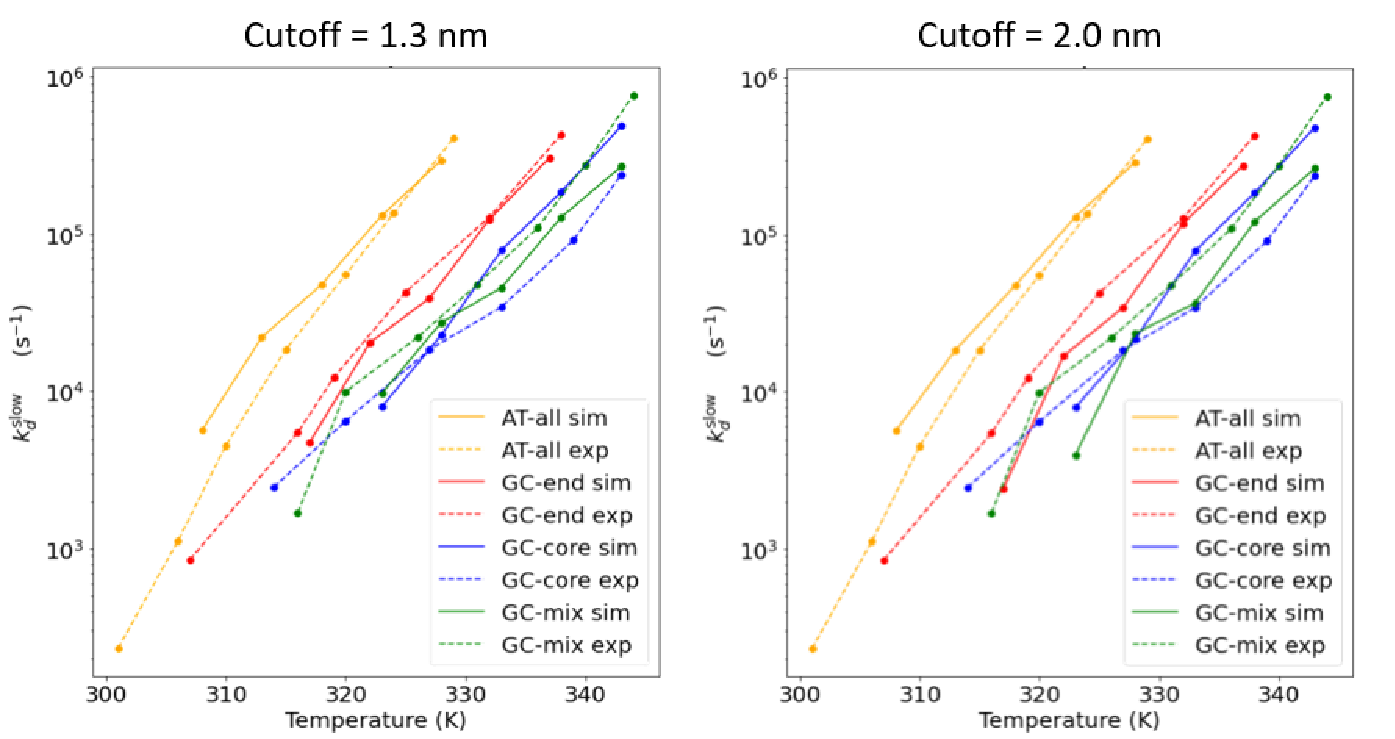
\includegraphics[width=\textwidth]{../FigR1.pdf}
        \caption*{\textbf{Figure R1.} Comparing the experimental slow response when increasing the cutoff parameter from 1.3 nm to 2.0 nm}
        \label{fig:compare_cutoffs}
	\end{center}
\end{figure}

We have modified the relevant text in Section 3.1 on p.~15 to read:

``First, we tracked the slow response corresponding to duplex dissociation in our simulations by compiling the distribution of times at which both of the central base pairs first separate to a distance of 1.3 nm starting from an initial fully hybridized duplex. This cutoff was selected as the distance beyond \rood{which} the strands are effectively non-interacting and define the dissociated state. \rood{We verified that our results were robust to choices of this cutoff over the range 0.8-2.5 nm.}''




\textcolor{blue}{5. The authors refer to "exponential" increase in Fig. 1. However, it's hard to see that an increase is exponential by eye unless the data is plotted on a log scale.}

\textbf{Author Reply:}   We agree that a log-linear plot would better expose these trends. We have replotted Fig.~1a and Fig.~S4 on log-linear axes and reproduce these below.

\begin{figure}[ht!]
	\begin{center}
        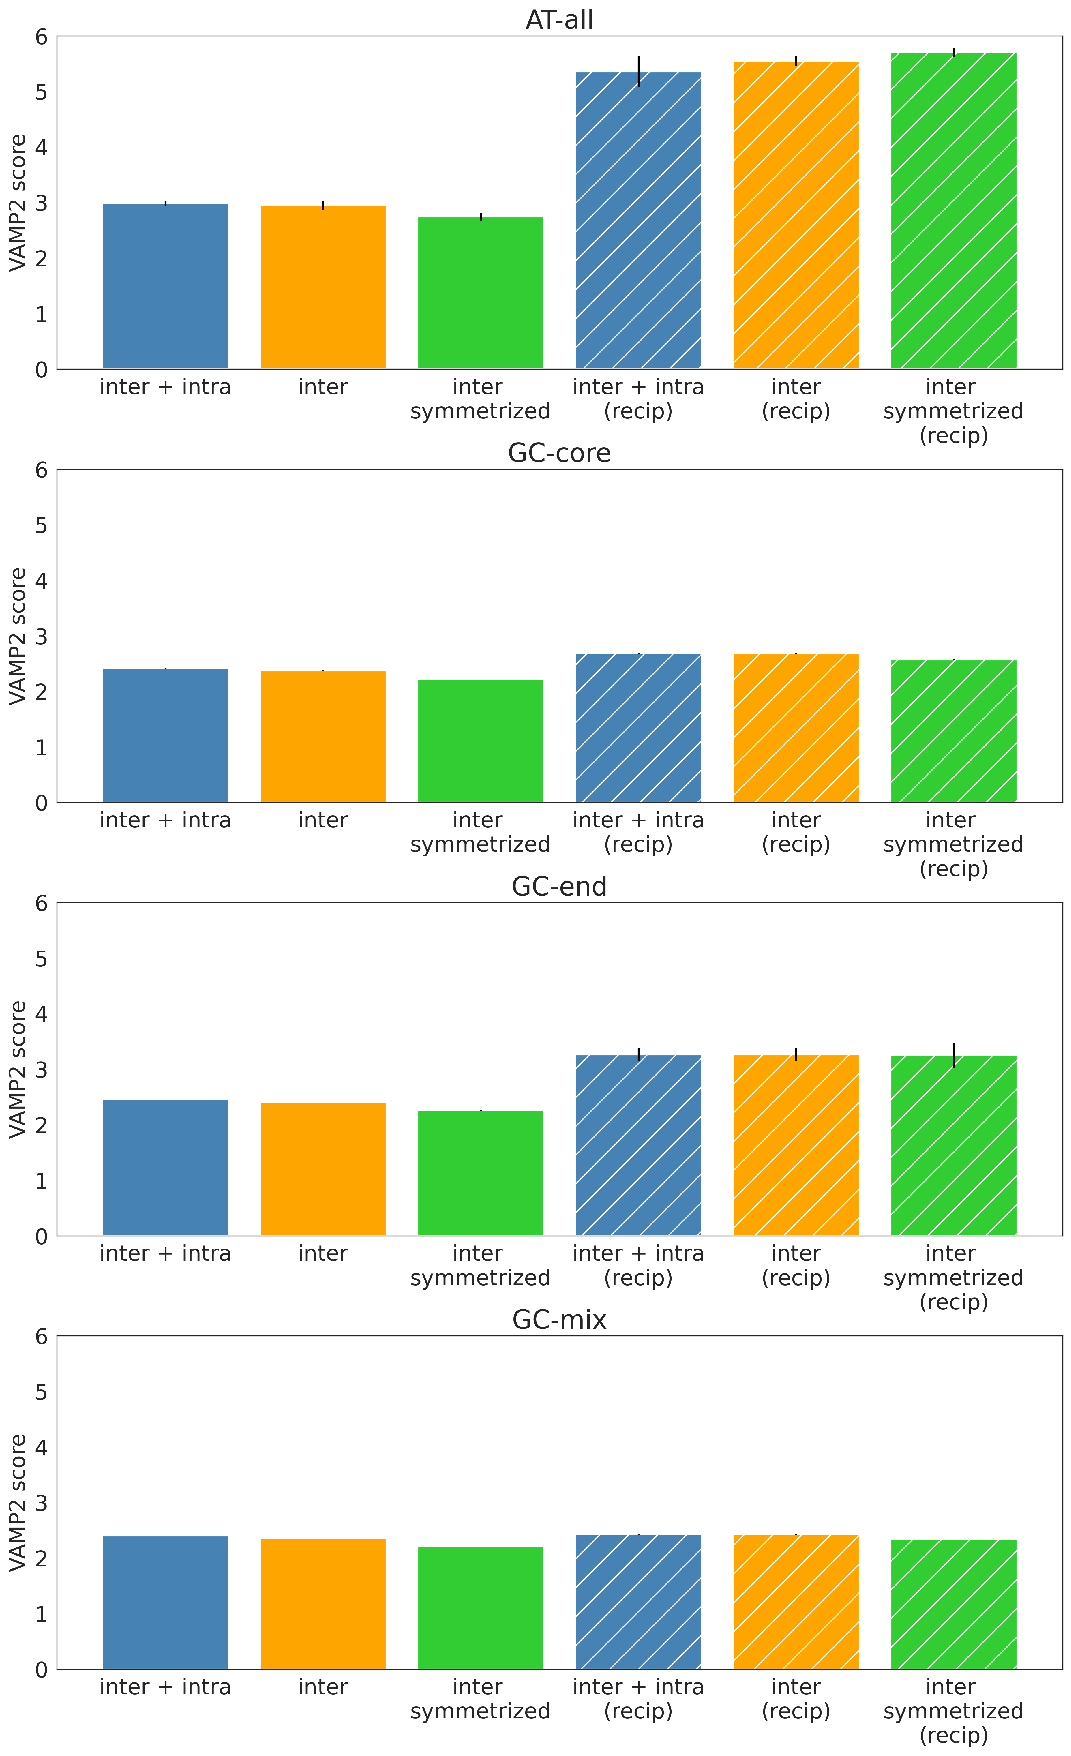
\includegraphics[width=1.0\textwidth]{../Fig1.pdf}
        \caption*{\textbf{Figure 1.} Experimental measurements and computational predictions of slow and fast at T-jump IR responses. Results are reported in terms of the final T-jump temperature. (a) The experimental and simulated slow rate constants $k_d^\mathrm{slow}$ corresponding to duplex dissociation over long time scales. \rood{We apply a fluctuation correction proposed by Ouldridge et al.\citep{Ouldridge2010ExtractingSimulations} to account for finite-size effects and ensure an asymptotically correct dimer fraction at long times.} (b) The experimental and simulated fast rate constant $k_d^\mathrm{fast}$ corresponding to terminal base-pair fraying on short time scales. The simulation results are corrected by a sequence-independent scaling factor that corrects for a 10$\times$ acceleration of the slow dissociation dynamics and 120$\times$ acceleration of the fast fraying dynamics. The simulated temperature in all cases is subjected to a (+4) K corrective calibration to account for an observed systematic under-prediction of the melting temperature by the 3SPN.2 model}
        \label{fig:relaxation-comparison_2}
	\end{center}
\end{figure}

\clearpage
\newpage

% Fig. S4
\begin{figure}[ht!]
	\centering
    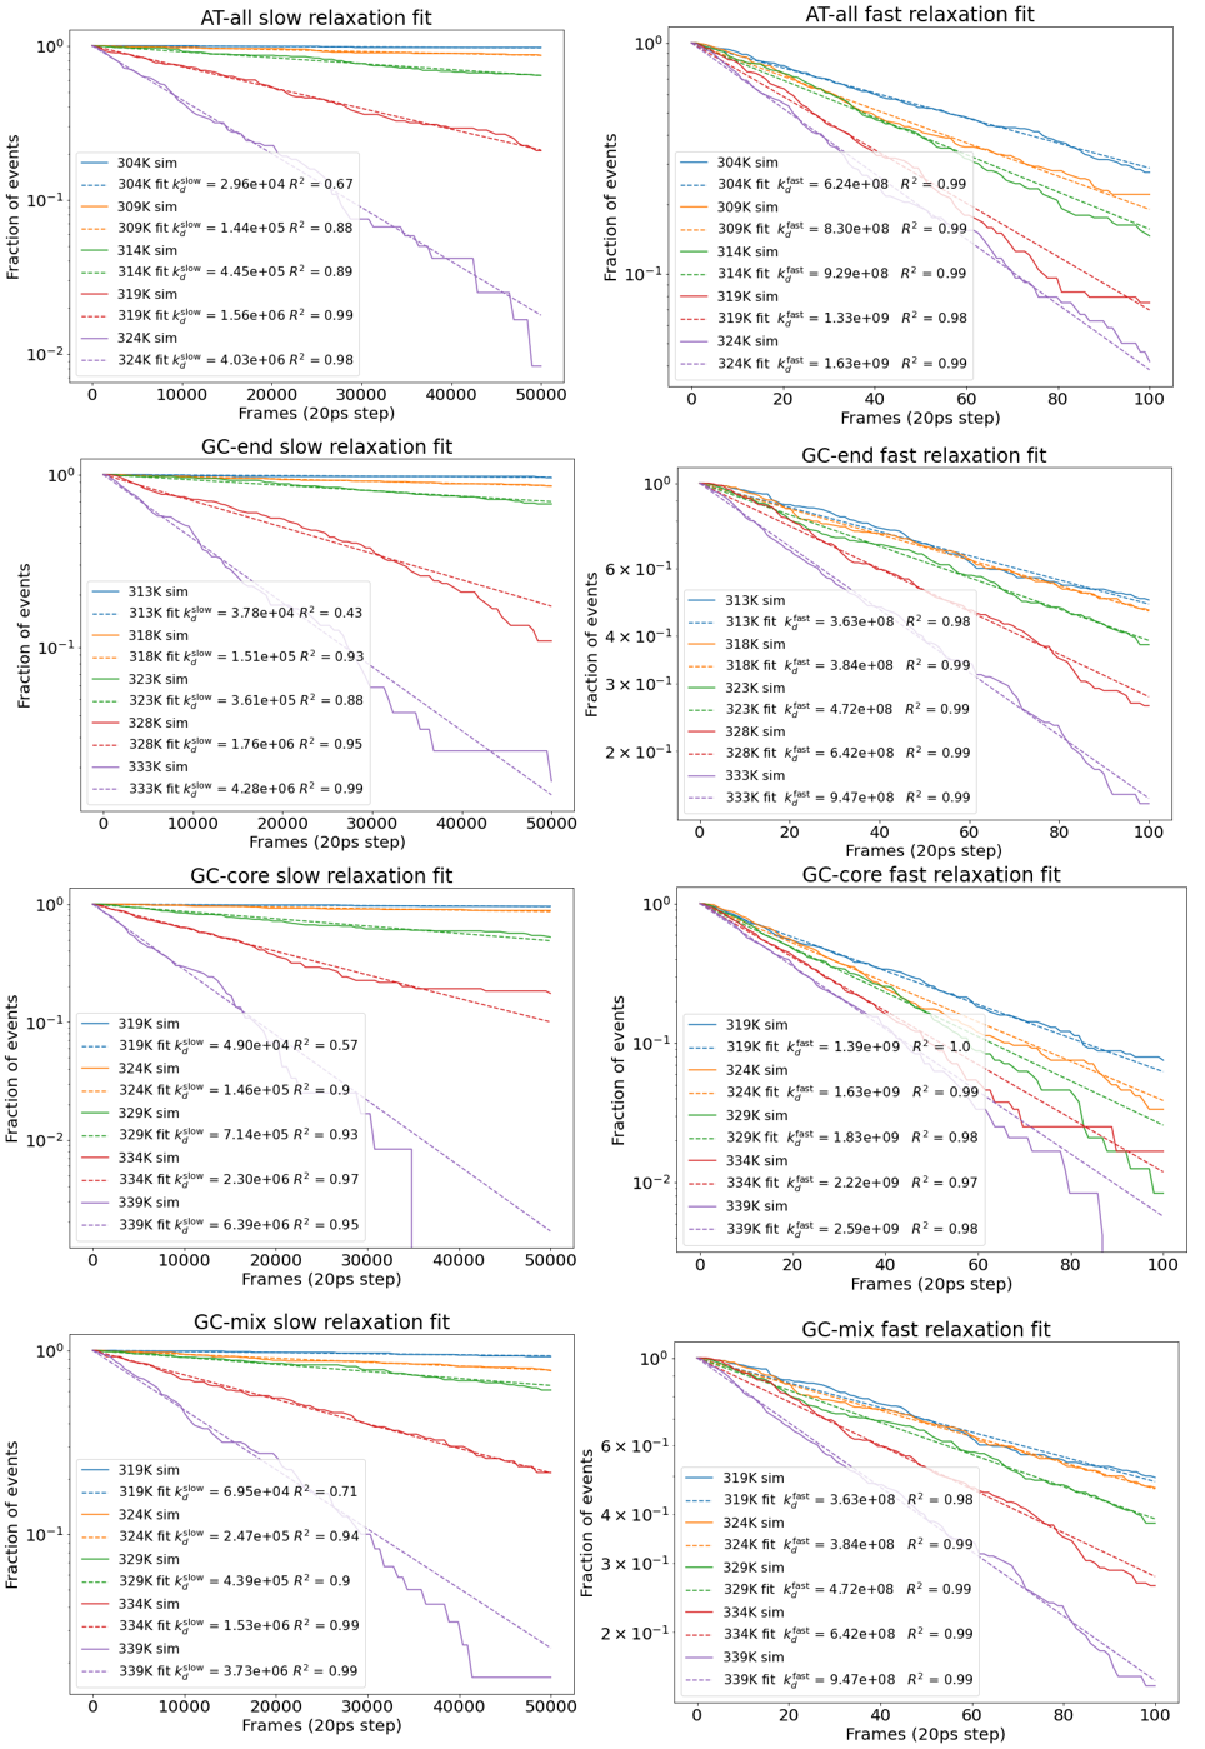
\includegraphics[width=.8\textwidth]{../FigS4.pdf}
   \caption*{\textbf{Figure S4.} Exponential fits for both slow (dissociation) and fast (fraying) response for all four sequences during ``computational T-jump'' experiments. From 120 independent 1 $\mu$s simulations, we compiled the slow response data by recording the fraction of sequences with both central Watson-Crick base pairs intact as a function of time, and the fast response data as the fraction of sequences with both terminal Watson-Crick base pairs intact as a function of time. We define a Watson-Crick base pair to be intact if the centers-of-mass of the two comlementary bases lie within a linear distance of 1.3 nm. We extracted our computational estimate of $k_d^\mathrm{fast}$ by fitting a decaying exponential to the fraction of bound A:T termini as a function of time $f_\mathrm{unfrayed}(t) = \exp(-k_d^\mathrm{fast}t)$. Similarly, we extracted our computational estimate of $k_d^\mathrm{slow}$ by fitting a decaying exponential to the fraction of hybridized sequences as a function of time $f_\mathrm{hybridized}(t) = \exp(-k_d^\mathrm{slow}t)$. \rood{We report within the figure legend to each panel the coefficient of determination $R^2$ for a least squares linear fit of the model to the data in log space (i.e., $\log \left( f \right) = -k_d t$) and data are plotted on log-linear axes to facilitate visual comparison of the fits. In all cases we observe excellent fits of the models to the data with all $R^2$ > 0.88 except for the slow response at the the lowest temperature T$_m$-5K where dissociation events are sparse.}}
    \label{fig:SIFig4_2}
\end{figure}

\clearpage
\newpage




\textcolor{blue}{6. Do the authors have any data on the scaling of k\_hybridization with T? In experiment, rates appear to increase with temperature (albeit with a much weaker dependence than de-hybridization rates). Simple "nucleation and zipper" models would predict the opposite, as does the oxDNA model (see ref 52).}

\textbf{Author Reply:}   This is an interesting question and are, in fact, considering embarking upon some additional work in this vein. Rigorous engagement of this question would require us to fit MSMs at a variety of temperatures in order to compare the pathways, mechanisms, and rates for hybridization and dehybridization. In the present work, we have only constructed MSMs at the melting temperature of each sequence and the collection of sufficient data to parameterize MSMs at other temperatures would require both (i) a substantial investment of time to collect the $\sim$1 ms of data required to fit robust MSMs and (ii) the use of biasing techniques in order to adequately sample hybridization (dehybridization) events at large temperature excursions above (below) the melting temperature. As such, we do not have the necessary data to engage this question at the present time. 

Reviewer \#2 raised a related point in their Comment \#2 and in response to both of these points, we have made the following modification to the terminal paragraph of the Conclusions on p.~38 observing that this may be an interesting follow-up study:

``Going forward, we will extend this work to discern more general trends in sequence-dependent hybridization/dehybridization for a wider range of oligomer sequences and motivate strategies for experimental comparisons. \rood{We also suggest that the MSM approach followed in this work, possibly coupled with biased sampling and reweighting techniques \citep{Wu2014StatisticallyStates, Scherer2015PyEMMAModels}, may be well-suited to expose changes in the hybridization/dehybridization mechanism and kinetics as a function of temperature.}''



\textcolor{blue}{7. The authors could explain a bit more carefully (perhaps in the SI) how they handle the multiple nearest-neighbour states that correspond to their microstates (eg. F4 clearly involves more than one NN configuration).}

We have modified the text in the ``Nearest neighbor model of duplex thermodynamics'' text in the Supporting Information to better describe for the reader how we performed this calculation. Specifically, we have appended the following text at the end of this discussion:

``\rood{In applying the NN model to each macrostate, we made the simplifying assumption that the ensemble of microstates constituting each macrostate could be represented by a single pattern of Watson-Crick base pairing that are schematically illustrated in Fig.~2a. In reality, each macrostate is composed of an ensemble of microstates that may have slightly different base pairing patterns and explicitly averaging over all of these microstates may change the predictions of the NN model. Recalculating the NN predictions by explicitly averaging over all microstates in the macrostate leads to changes in the $\Delta F = F - F_H$ values reported in Fig.~3 (i.e., the free energy of each macrostate relative to the hybridized state) of $<$1 kJ/mol. As such, representing each macrostate by a single representative microstate and base pairing pattern is a highly accurate simplifying approximation for the purposes of this calculation.}''

\textcolor{blue}{8. I don't understand how the population of F4 could be >50\% that of H for the GC-core system, when the free energy of F4 is reported as > 5kJ/mol. My back-of-the-envelope maths predicts a ratio of 8:1 for a 5kJ/mol gap. Incidentally, 8:1 is roughly the ratio I got from running the configurations through NUPACK.}

\textbf{Author Reply:}  We apologize for the confusion and have resolved the origin of this apparent inconsistency to two factors: (i) a unit conversion error on our part and (ii) our choice to present the bar plots in Fig.~2b on a log axis.

(I) First, we made an (embarrassing) unit conversion error in reporting the $\Delta F$ value for the F4 state of the GC-core sequence from our MSM model. Specifically, we did not convert the $\Delta$F from units of $kT$ at $T_m$ = 324 K to kJ/mol, resulting us to erroneously report a value of 5.1 kJ/mol instead of 5.1 $kT$ = 13.7 kJ/mol. Using this correct $\Delta$F value we see agreement between the reported free energy in Fig.~3 and populations reported in Fig.~2. We can demonstrate this by performing the same back-of-the-envelope verification proposed by the reviewer:

\begin{itemize}
\item $G_H$ = $G_D$ = 0 (adopting this as the arbitrary zero of free energy and asserting that the sequence is at its melting temperature so the hybridized H and dissociated D states are equiprobable)
\item $G_{F4}$ = 5.1 $kT$ at $T_m$ = 324 K = 13.7 kJ/mol
\item $f_H$ + $f_D$ + $f_F$ = 1 (the fractional populations sum to unity)
\item $f_X$ = $\exp (-\beta G_X$) / $Z$ ($Z$ is the partition function that imposes normalization)
\end{itemize}

We can solve this system of equations to yield $f_{F4}$ = 0.0030 that is in excellent agreement with the MSM predictions of $f_{F4}$ = 0.0028 that we report in Fig.~2b. 

We have updated Figure 3 with the correct $\Delta$F as shown below.

\begin{figure}[ht!]
	\begin{center} 
        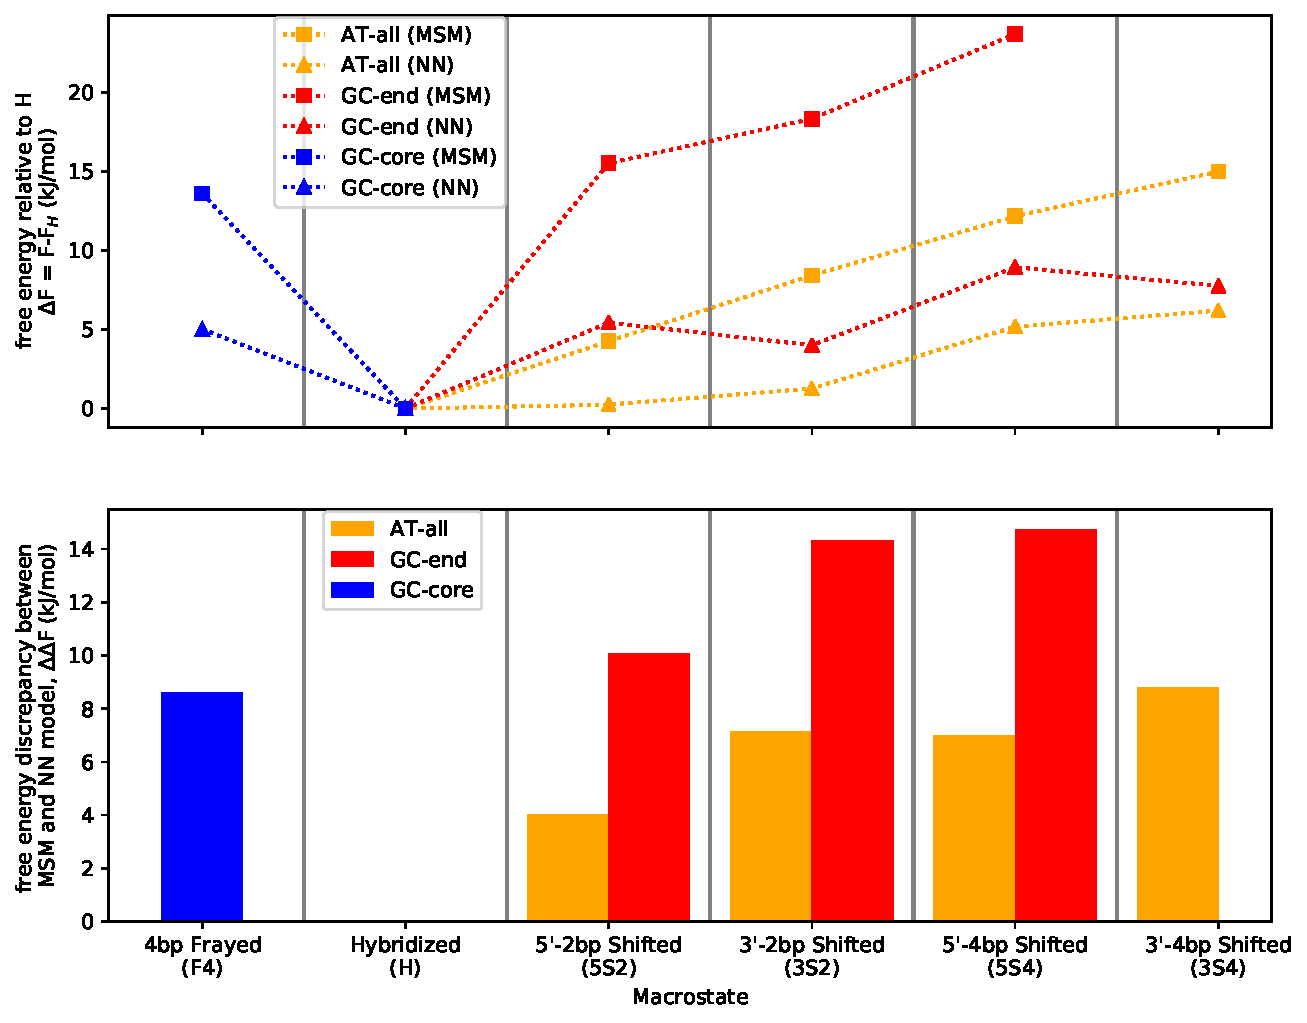
\includegraphics[width=140mm, scale=1]{../Fig3.pdf}
        \caption*{Figure 3. Comparison of the macrostate free energy predictions of the MSMs and nearest neighbor (NN) thermodynamic model \rood{at the sequence melting temperatures}.~\citep{SantaLucia1998AThermodynamics, Santalucia2004TheMotifs} (a) Free energies of each macrostate relative to the hybridized state $\Delta F = F - F_H$. We define the hybridized state H to possess a free energy of zero and take care to only compare relative free energies (i.e., $\Delta F$) between the MSM and NN model. (b) Discrepancy between the macrostate relative free energy predictions $\Delta \Delta F = \Delta F^\mathrm{MSM} - \Delta F^\mathrm{NN}$ of the MSM relative to the NN model. The MSM tends to predict higher relative free energies (i.e., lower occupancy probabilities) relative to the hybridized state H compared to the NN model.}
        \label{fig:NN_table}
	\end{center}
\end{figure}

We have also updated the second paragraph of Section 3.3 on p.~23 as follows:

``As illustrated in Fig.~3, we see that the MSM tends to predict higher free energies for \rood{all macrostates relative to the H state compared to the NN model}. Although the trends are in qualitative agreement, what is the root of the quantitative discrepancy of the MSM and NN models in the predicted relative stabilities?''

We recognize that this was a significant miscalculation, and we have re-checked all free energy results to ensure that (i) we did not make a similar error for any of the other reported values in Fig.~3 or anywhere else and (ii) that this error did not propagate through to any subsequent calculations, results, or conclusions within the remainder of the manuscript.



(II) We also note that our choice of a logarithmic y-axis for the bar plots in Fig.~2b that make the bar associated with the F4 state appear nearly 50\% of the height of the H and D bars for GC-core. We made this plotting choice in order to make visible on these bar plots the small state populations associated with the shifted and frayed states and noted the percentage occupancies on the bars themselves. To help eliminate this confusion, we have modified the portion of the Fig.~2 caption referring to this panel to read: 

``(b) \textbf{Thermodynamics.} Histograms reporting the number of the $10^7$ total frames within the 1 ms of simulation trajectories observed to occupy each of the seven macrostates, corresponding to our numerical estimates of the equilibrium occupancy probabilities. Uncertainties are calculated across 100 MSMs using a Bayesian MSM estimation are reported for each bar and are very small compared to the total counts. \rood{Values are reported on a log y-axis to make the small populations of the shifted and frayed states visible.}''




\textcolor{blue}{9. Is the MSM model explicitly constrained to obey detailed balance? The numbers that come out seem consistent with detailed balance - forward and backward trajectories at the same T essentially look the same (they're equally likely to go through intermediates). This should be a feature of the MSM, but it's unclear to me whether it's hard-coded or just arises naturally in the coarse-graining.}

\textbf{Author Reply:}    The reviewer raises a good point regarding the assumptions made during MSM construction. We do indeed use a reversible MSM framework that enforces detailed balance. This is an important point which we have now made explicit by modifying the text in Section 2.1.2 on p.~11 to read:

``The 200 microstates comprising each system were coarsened into our terminal macrostate MSM. \rood{Since we are interested in the construction of models of the equilibrium kinetics, we explicitly enforce detailed balance in the construction of the MSM. \citep{Wehmeyer2019IntroductionSoftware}}''

and the text in Section 3.4 on p.~26 to read:

``In addition to thermodynamic stabilities, the macrostate MSM also furnishes quantitative and interpretable predictions of hybridization and dehybridization pathways and mechanisms \rood{at the sequence melting temperatures}. \rood{It should be noted that because we are using a reversible MSM framework, detailed balance is enforced by construction.}''



\textcolor{blue}{Relatedly, some of the discussion of the hybridization and de-hybridization pathways in non-repetitive sequences seems to ignore this fact. In these equilibrium simulations, hybridization trajectories played in reverse should be statistically indistinguishable from de-hybridization trajectories. I don't think anything that's said is wrong, per se, but it might be worth considering how the contrast between "nucleation and zippering" and "fraying-peeling" is consistent with the symmetry in the pathways.}

\textbf{Author Reply:}  This is a nice observation, and we would do well to note this symmetry for the reader. We have added a sentence to this effect in Section 3.6 on p.~32:

``In dehybridization, we observe fraying \rood{of one half of the duplex with the strands remaining associated until the loss of the final A:T pairs and ultimately the last G:C pair}. Qualitatively, we observed some short-lived states composed of two to four native WC base pair contacts immediately before full dissociation occurs, but, in contrast to the F4 state we observe in GC-core, these conformations do not constitute a metastable state within our MSM nor do they tend to reform intact duplexes. These dissociation dynamics are consistent with a ``fraying-peeling'' dehybridization mechanism.\citep{Wong2008TheSimulations, Perez2010Real-timeUnfolding, Zgarbova2014BaseRNA} \rood{We observe that the principle of microscopic reversibility for a molecular system at thermodynamic equilibrium imposes the conditions of detailed balance and symmetry of the classical equations of motion under time reversibility \cite{McCully2008MicroscopicHomeodomain}. A consequence of these considerations is that if our system is indeed at equilibrium, then the ``fraying-peeling'' dehybridization mechanism can be considered a reversal of the ``nucleation-zippering'' hybridization pathway since the time-reversed simulation trajectories represent an equally valid sampling of the system dynamics. This is indeed borne out by our mechanistic observations for GC-mix wherein the early stages of ``nucleation-zippering'' proceed by the formation of one G:C contact followed by one or more additional A:T pairs and the late stages by the formation of all remaining WC pairs, which we compare with the early stages ``fraying-peeling'' wherein one half of the duplex frays and the late stages wherein dissociation finally completes by the dissolution of the last few A:T contacts and the final G:C pair.}''



\textcolor{blue}{10. I think some of the characterisation of the "all or nothing" picture is a bit misleading. The two state model of duplex formation is really a thermodynamic model, based on the assumption that the ensemble of hybridized and de-hybridized states look very different and are separated by a large barrier. This model is perfectly consistent with the transition between the two ensembles involving a complex network of metastable states. Indeed, as the authors note on line 3 of p4, a number of previous authors have considered what such states might look like, particularly for repetitive sequences. The authors' primary contribution here is not proposing that these states exist for the first time, but trying to tie together evidence from simulation and experiment to describe them.}


\textbf{Author Reply:}   We thank the reviewer for this important observation and illuminating our need to better clarify this potentially ambiguous concept. We have modified the text in Section 3.6 on p.~29 to read:

``The GC-mix sequence is the only one of the four sequences studied that exhibits simple two-state ``all-or-nothing'' behavior.~\citep{Xiao2019, Araque2016LatticeCooperativity, Sikora2013ModelingIntermediates, Sanstead2016} \rood{This characterization is intended to reflect that the mechanistic observation that} GC-mix MSM comprises just two states, the hybridized H and dehybridized D (Fig.~2c), indicating that association and dissociation of the strands proceeds directly without passing through any metastable intermediate states resolvable under the $\tau$=1.2 ns lag time of our MSM. \rood{Indeed, the sequence's propensity to fray in simulation and the role of termini fraying in dissociation experiments \citep{Sanstead2016} indicate that there remain deviations from ``all-or-nothing'' behavior which are not fully captured within the MSM lag time. (We note that ``all-or-nothing'' can also be used, somewhat ambiguously, to refer to a two-state thermodynamic model where the hybridized and dehybridized are separated by a large free energy barrier but that the transitions between them may proceed through a network of metastable states.)}''

We have also removed ``all-or-nothing'' from the experimental methods section as the fitting procedure is more appropriately described as simply ``two-state'' so that the relevant text in Section 2.2.3 on p.~14 now reads:

``FTIR temperature series were measured for each sequence as reported previously,~\citep{Sanstead2016} and the second SVD component along temperature was fit to a \rood{two-state model} to determine the fraction of intact duplex $\theta$ as a function of temperature.''



\textcolor{blue}{11. Related to the above, the references on line 3 of p4 should probably also include Ref 52, where a similar analysis of metastable states in a repetitive sequence is performed (for a different coarse-grained model) and [Flamm, W., Fontana,J.M., Hofacker, I.L. and Schuster,P. (2000) RNA folding at elementary step resolution. RNA, 6, 325-338] where a defect diffusion mechanism is proposed.
}

\textbf{Author Reply:}   We have added these references to those at the top of p.~4.


\textcolor{blue}{12. The reasoning behind why the broader relaxation spectrum is indicative of misaligned states was not that clear to me. Why would "elevated" fraying cause a broader response? Wouldn't it also, then, be broader for CG-core, which has elevated fraying? It seems to me that the argument is more along the lines of the heterogeneity of the configurations leading to heterogeneous dynamics, and hence a broader relaxation profile. But I am no expert on this technique.}

\textbf{Author Reply:}   The reviewer makes a good comment on our choice of language used to described the stretched AT-all response. It is indeed our contention that the heterogeneity of the configurations in the initial ensemble and the fraying dynamics exhibited in each of these states that is the origin of the broadening of the relaxation profile, but our wording here was insufficiently clear. We believe that the reviewer's phrasing ``heterogeneity of configurations leads to heterogeneous dynamics'' expresses this idea much more clearly and we have integrated it into our edits of Section 3.7 on p.~33:

``Nevertheless, the presence of these out-of-register shifted states in the low-temperature equilibrium ensemble prior to the T-jump step may be observable via their influence on the fast T-jump IR response attributable to fraying. Specifically, we hypothesize that the dangling ends and inert tails present in the out-of-register shifted states should promote an \rood{elevated fraying response over the course of the relaxation that is distinct from that of in-register fraying. This heterogeneity of configurations should lead to heterogeneous dynamics, manifested in the observation of a more stretched relaxation over experimental time scales of 70-100 ns.} Analysis of the MSM equilibrium distributions reveals 10.0\% of the equilibrium ensemble to reside in out-of-register shifted states 3S2, 5S2, 3S4, and 5S4 for AT-all, compared to just 0.23\% for GC-end, and 0\% for GC-core and GC-mix. It is our conjecture that a substantial population of out-of-register shifted states in the pre-T-jump AT-all ensemble should be distinguishable from the GC-end, GC-core, and GC-mix as an elongation of the fast relaxation response associated with terminal base fraying.''


\textcolor{blue}{13. How much of the code is being made available? Ideally, the initialization files for the simulations and the code used to perform the MSM analysis would be publicly available. Additionally, it would be good to publish the raw experimental data and the processing tools used to obtain the final results.}

\textbf{Author Reply:}   We have uploaded input files and analysis scripts to Github (\url{https://github.com/mrjoness/Oligo-MSMs}) and 45 GB of featurized trajectories and experimental data to Zenodo (\url{https://doi.org/10.5281/zenodo.5140040}). The links to both of these resources are now noted in the Supporting Information statement on p.~38:

``\rood{Input files and analysis scripts have been uploaded to Github (\url{https://github.com/mrjoness/Oligo-MSMs}) and 45 GB of featurized trajectories and experimental data to Zenodo (\url{https://doi.org/10.5281/zenodo.5140040}).}''




\clearpage
\newpage

\begin{shaded}
\textbf{Additional editorial edits}
\end{shaded}

\textcolor{blue}{1. Please include at least the first page for each reference citation for the following incomplete journal reference 48}

Updated.

\textcolor{blue}{2. Please update the publication status of reference 70, if possible.  Providing the DOI is acceptable.}

We are unable to locate any additional citation information beyond the arXiv link.

\textcolor{blue}{3. Please include publisher for the following incomplete book reference: 79.}

Updated.

\textcolor{blue}{4. The TOC graphic should fit in an area no larger than 3.25 in. by 1.75 in. (approx. 8.25 cm by 4.45  cm) and should have adequate resolution and clarity. Confirm that all text is legible at this size.}

Updated and confirmed.


\clearpage
\newpage

\bibliographystyle{achemso}
\bibliography{../references_210514_abv}
\end{document}
